\documentclass[aspectratio=169,compress,x11names]{beamer}
\usefonttheme[onlymath]{serif}
%\setbeameroption{show notes on second screen}
\setbeameroption{hide notes}
\usetheme{Boadilla}
	\setbeamertemplate{navigation symbols}{}
	\setbeamertemplate{headline}{%
	\leavevmode%
	\hbox{%
		\begin{beamercolorbox}[wd=\paperwidth,ht=2.5ex,dp=1.125ex]{section in head/foot}%
			\insertsectionnavigationhorizontal{\paperwidth}{}{\hskip0pt plus1filll}
		\end{beamercolorbox}%
	}%
	\vspace*{-1em}  % Giảm khoảng trống phía dưới thanh điều hướng
}
\usepackage{tikz-feynman}
\usepackage{array}
\usepackage{animate}
\usepackage{amsmath,nicematrix,esint}

\usepackage{cancel}
\usepackage{multicol}
\usepackage{physics}
\usepackage{xcolor}
\usepackage{graphicx,subcaption}
\usepackage{amssymb}
\usepackage{hyperref}
%\hypersetup{colorlinks = true,linkcolor = black,filecolor= black,urlcolor= black}
\usepackage{cancel}
\usepackage{subcaption}
\usepackage{comment}

\usepackage[backend=bibtex,bibencoding=utf8,doi=false,isbn=false,url=false,eprint=false,indexing=false,bibstyle=authoryear,citestyle=authortitle-icomp]{biblatex}
\addbibresource{../refs.bib}
\AtEveryBibitem{%
	\clearname{translator}%
	\clearlist{publisher}%
	\clearfield{pagetotal}%
}
\setbeamertemplate{bibliography item}{}


\newcommand{\biblion}[3]{
	\bibitem{}  
	#1, {\color{black}\textit{#2}}, {\color{LightSteelBlue3}#3} \\
}



\makeatletter
\renewcommand\@makefnmark{\hbox{\@textsuperscript{\usebeamercolor[fg]{footnote mark}\usebeamerfont*{footnote mark}[\@thefnmark]}}}
\renewcommand\@makefntext[1]{{\usebeamercolor[fg]{footnote mark}\usebeamerfont*{footnote mark}[\@thefnmark]}\usebeamerfont*{footnote} #1}


\makeatother


\usepackage{xparse}

\usepackage[toc,page]{appendix}
\author{Tran Khoi Nguyen}
% Title page details: 
\author[Presenter: Tran Khoi Nguyen]{{\textit{Presenter}} \\
	Tran Khoi Nguyen \inst{1} \\
	{\and} \\
	{\textit{Supervisor}} \\
	Dr. Huynh Thanh Duc \inst{2}}
\institute[HCMUS]{\inst{1} University of Science, Ho Chi Minh city\and %
	\inst{2} Institute of Applied Mechanics and Informatics}
% Title page details: 
\title[Hofstadter butterfly of TMD]{Hofstadter butterfly in transistion metal dichalcogenide monolayers}
	
\date{Jul, 2025}
\logo{\includegraphics[height=0.9cm]{pic/logo1.png}\vspace*{-.055\paperheight}\hspace*{.85\paperwidth}}
\newcommand{\at}[2]{\bigg\rvert_{#1}^{#2} }

\begin{document}
	\setbeamertemplate{logo}{}
	\begin{frame}
		\titlepage
		\vspace*{-0.6cm}
		\begin{figure}[htpb]
			\begin{center}
				
\includegraphics[keepaspectratio, scale=0.02]{../pic/logo.png}
				\includegraphics[keepaspectratio, scale=0.02]{../pic/logo1.png}
			\end{center}
		\end{figure}
	\end{frame}
	\logo{}
	\begin{frame}{Table of Contents}
		\tableofcontents
		\note{note text}
	\end{frame}
	\section{Overview}
	\begin{frame}{Overview}
		Group VI-B Transition Metal Dichalcogenides (TMD) are compound semiconductors of the type MX$_2$
		\begin{figure}
			\centering
			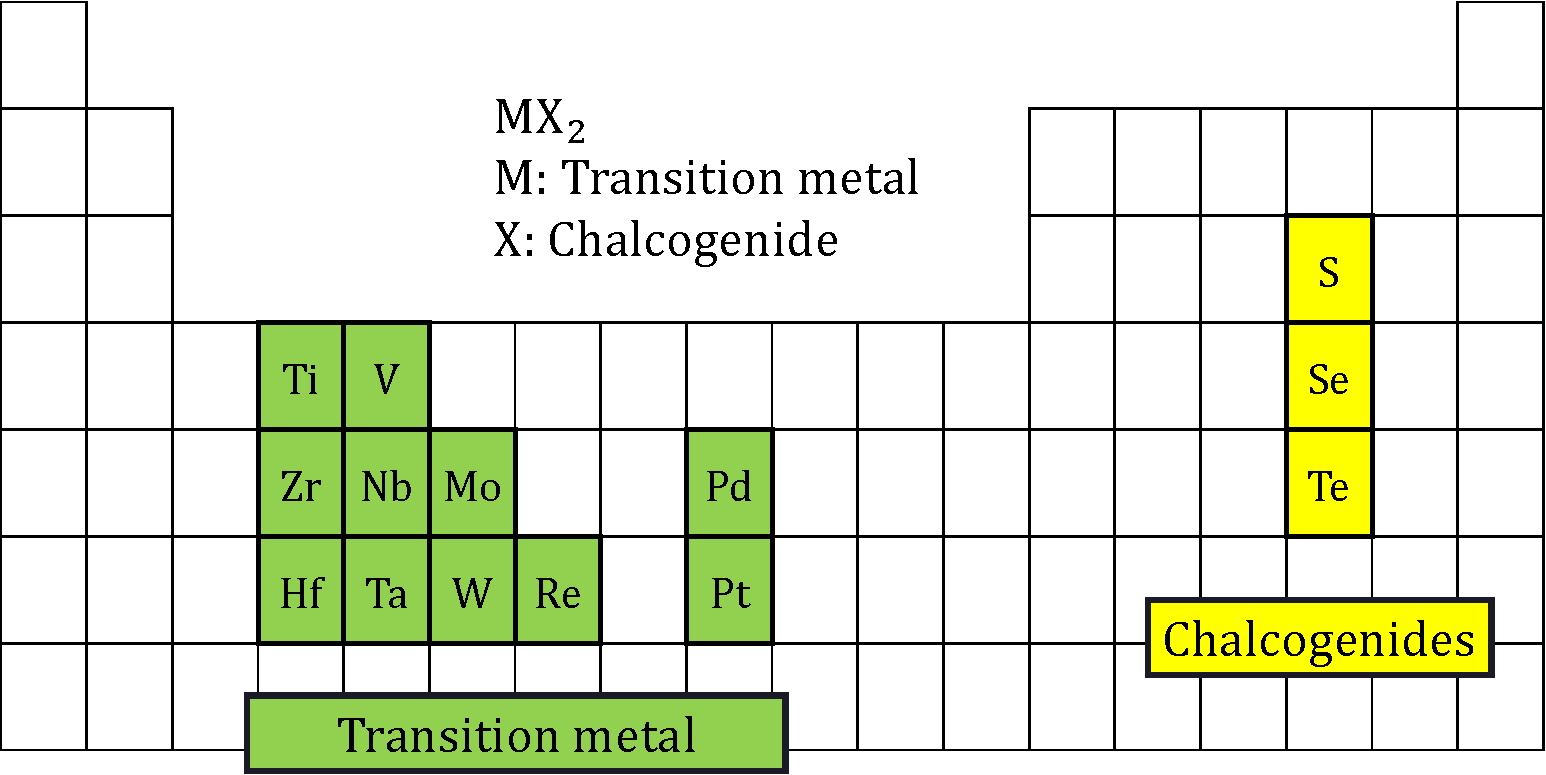
\includegraphics[width=0.65\linewidth]{./pic/periodictable.pdf}
			\caption{Transition metal dichalcogenides compound.}
		\end{figure}
	\end{frame}
	\begin{frame}{Transition Metal Dichalcogenides Monolayers}
		\begin{multicols}{2}
			\begin{itemize}
				\item One $\color{green}M$ layer sandwiched by two $\color{yellow}X$ layers as show in top view (a) and side view (b).
				\item Crystal structure has no central inversion symmetry.
				\item The symmetry of the lattice results in the hexagon Brillouin Zone (BZ).
			\end{itemize}
			\columnbreak
			\vfil
			\begin{figure}
				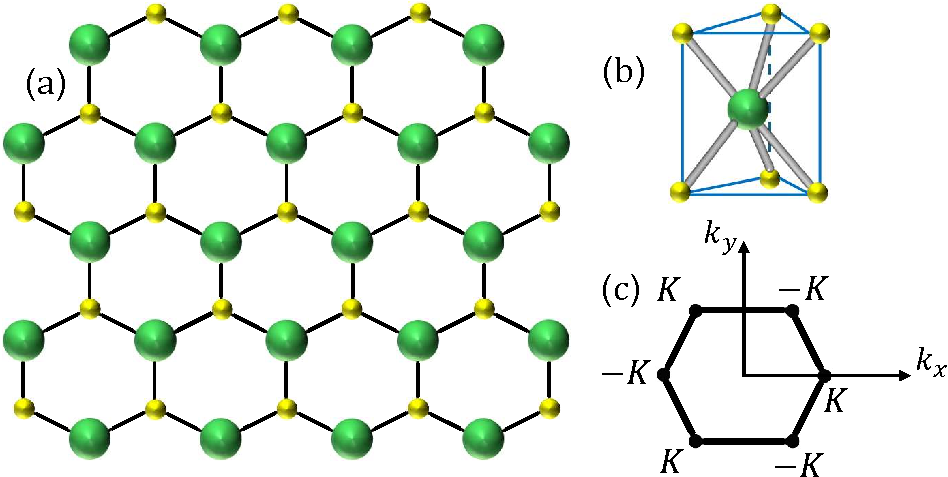
\includegraphics[width=\linewidth]{./pic/latticePresent.pdf}
				\caption{Structure and Brillouin Zone of Monolayer TMD\footcite{PhysRevB.88.085433}.}
			\end{figure}
		\end{multicols}
	\end{frame}
	\begin{frame}{Transition Metal Dichalcogenides Monolayers}
		\begin{block}{Properties}
			\begin{itemize}
				\item Both mono-layer and few-layers remain stable at room temperature.
				\item TMD monolayer has the visible band gap in the ban structure, which can be used in creating the transistor devices\footnotemark.
				\item  Strong spin-orbit coupling (SOC) in TMD monolayers lead to spin splitting of hundres meV.
			\end{itemize}
		\end{block}
		$\Rightarrow$ Promising material in electronic and optoelectronic applications.
		\footnotetext{\cite{radisavljevic2011}}
	\end{frame}
	\section{Method}
	\subsection{Three-band tigh-binding model without magnetic field}
	\begin{frame}{Three-band tigh-binding model without magnetic field}
		Time-independent Schr\"{o}dinger equation for an electron in the crystal
		\begin{gather}
			\left[-\frac{\hbar^{2} \boldsymbol{\nabla}^{2}}{2m} + U_{0}(\mathbf{r})\right] \ket{\psi_{\lambda,\mathbf{k}}(\mathbf{r})} = \epsilon_{\lambda,\mathbf{k}} \ket{\psi_{\lambda,\mathbf{k}}(\mathbf{r})}.
		\end{gather}
		Tight-binding (TB) wave function
		\begin{gather}
			\ket{\psi_{\lambda,\mathbf{k}}(\mathbf{r})} = \sum_{j} C_{j}^{\lambda}(\mathbf{k}) \sum_{\mathbf{R}} e^{i \mathbf{k} \cdot \mathbf{R}} \ket{\phi_{j} (\mathbf{r} - \mathbf{R})}.
		\end{gather}
		The basis consists of three $d$-orbitals of the $M$ atom:
		\begin{gather}
			\ket{\phi_{1}} = \ket{d_{z^{2}}} , 
			\ket{\phi_{2}} = \ket{d_{xy}} , 
			\ket{\phi_{3}} = \ket{d_{x^{2} - y^{2}}}.
		\end{gather}
		The coefficents $C_{j}^{\lambda}(\mathbf{k})$ are the solutions of the eigenvalue equation
		\begin{gather}
			\sum_{jj'}^{3} \left[H_{jj'}^{\text{TB}}(\mathbf{k}) - \varepsilon_{\lambda}(\mathbf{k}) S_{jj'}(\mathbf{k})\right] C_{j}^{\lambda}(\mathbf{k}) = 0.
		\end{gather}
	\end{frame}
	\begin{frame}{Three-band tigh-binding model without magnetic field}
		Overlap matrix elements
		\begin{gather}
			S_{jj'}(\mathbf{k}) = \sum_{\mathbf{R}} \bra{\phi_{j}(\mathbf{r})} \ket{\phi_{j'}(\mathbf{r - R})} \approx \delta_{jj'}.
		\end{gather}
		TB Hamiltonian matrix elements
		\begin{gather}
			H_{jj'}^{\text{TB}}(\mathbf{k}) = \sum_{\mathbf{R}} e^{i \mathbf{k \cdot R}} \bra{\phi_{j}(\mathbf{r})} \left[-\frac{\hbar^{2} \boldsymbol{\nabla}^{2}}{2m} + U_{0}(\mathbf{r})\right] \ket{\phi_{j'}(\mathbf{r - R})}.
		\end{gather}
	\end{frame}
	\begin{frame}{Three-band tigh-binding model without magnetic field}
		\begin{figure}
			\centering
			\includegraphics[width=0.6\linewidth]{pic/bandstructureTNN.pdf}
			\caption{Band structure of MoS$_{2}$ monolayer\footcite{PhysRevB.88.085433}.}
		\end{figure}
	\end{frame}

	\subsection{Three-band tigh-binding model under a magnetic field}
	\begin{frame}{Three-band tigh-binding model under a magnetic field}
		TB Hamiltonian matrix elements change to
		\begin{gather}
			H= \frac{(-i \hbar \boldsymbol{\nabla} + e \mathbf{A}(\mathbf{r}))^{2}}{2m} + U_{0}(\mathbf{r}) + g^{*} \mu_{B} \mathbf{B} \cdot \mathbf{L},
		\end{gather}
		It is possible to add a phase factor to the basis functions
		\begin{gather}
			\psi_{\lambda,\mathbf{k}}(\mathbf{r}) = \sum_{j=1}^{3} C_{j}^{\lambda}(\mathbf{k}) \sum_{\mathbf{R}} e^{i \mathbf{k} \cdot \mathbf{R} } e^{i\theta_\mathbf{R}(\mathbf{r})} \phi_{j}(\mathbf{r} - \mathbf{R}).
		\end{gather}
		By choosing $\theta_\mathbf{R} = - \tfrac{e}{\hbar} \int_{\mathbf{R}}^{\mathbf{r}} \mathbf{A}(\mathbf{r'}) \cdot d\mathbf{r}' $ as Peierls substitution, the Hamiltonian matrix elements as the form
		\begin{equation}
			\begin{aligned}
				H_{jj'}^{\text{TB}}(\mathbf{k})
				&= \sum_{\mathbf{R}} e^{i\mathbf{k \cdot R}} e^{\frac{ie}{\hbar} \int_{\mathbf{0}}^{\mathbf{R}} \mathbf{A(\mathbf{r'})} \cdot d \mathbf{r'} } \bra{\phi_{j}(\mathbf{r})} \left[ -\frac{\hbar^{2} \boldsymbol{\nabla}^{2}}{2m} + U_{0} (\mathbf{r}) \right] \ket{\phi_{j'}(\mathbf{r - R})} \\
				&+ g^{*} \mu_{B} \mathbf{B} \cdot \sum_{\mathbf{R}} e^{i\mathbf{k \cdot R} + \frac{ie}{\hbar} \int_{\mathbf{0}}^{\mathbf{R}} \mathbf{A(\mathbf{r'})} \cdot d\mathbf{r'} } \bra{\phi_{j}(\mathbf{r})} \mathbf{L} \ket{\phi_{j'}(\mathbf{r - R})}.
			\end{aligned}
		\end{equation}
	\end{frame}
	\begin{frame}
		\begin{figure}
			\centering
			\includegraphics[width=0.5\linewidth]{./pic/siteindex_2_crop.pdf}
			\caption{\label{fig:site index} The TB model of TMDC with six neighbors atom $M$.}
		\end{figure}
	\end{frame}
	\begin{frame}{Three-band tigh-binding model under a magnetic field}
		\begin{multicols}{2}
			The Eq (9) is consist only 1-atom $M$ in the unit cell, and the Hamiltonian does not invariant under the expansion of lattice vector along the $x$ axis. In order to restore this invariance, we expanded the origin unit cell into a magnetic unit cell, which now contains $2$-atoms $M$.
			\columnbreak
			\begin{figure}
				\centering
				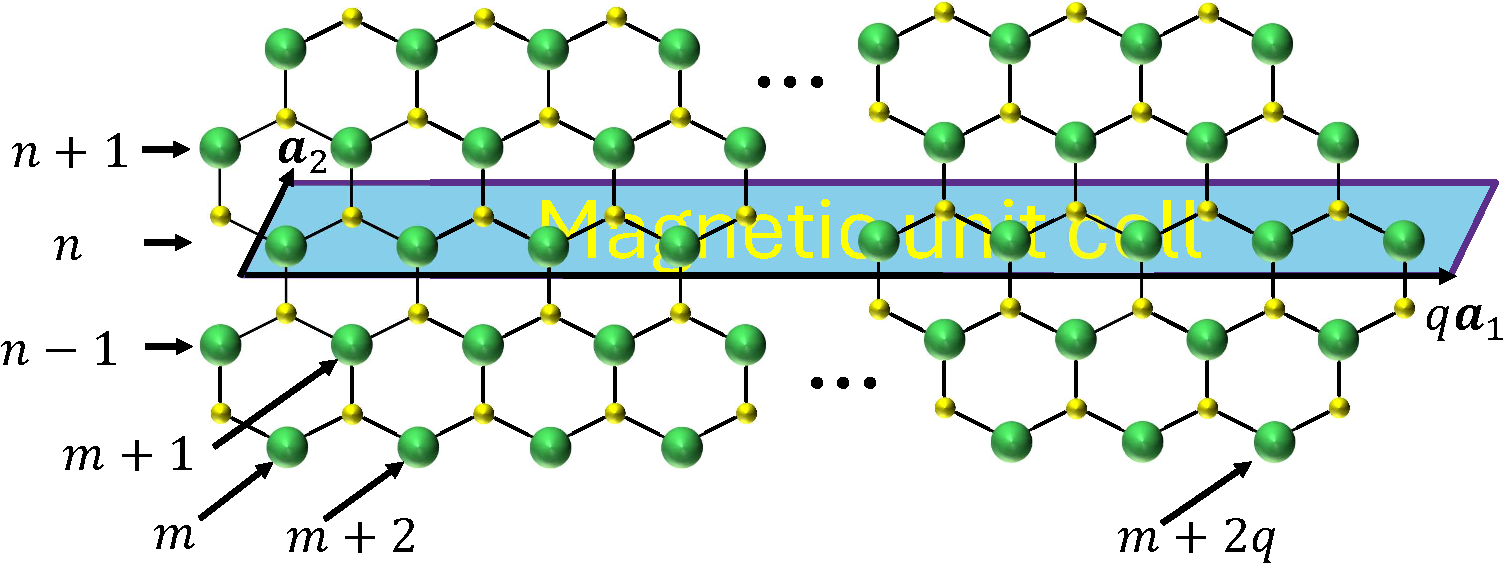
\includegraphics[width=\linewidth]{../pic/magneticUC_cut.pdf}
				\caption{\label{fig:Mag UC} Magnetic unit cell for TMD monolayers.}
			\end{figure}
		\end{multicols}
	\end{frame}
	\begin{frame}{Hamiltonian of magnetic unit cell}
		The new basis set of $6q$ atomic orbitals is defined as
		\begin{gather}
			\psi_{\lambda,\mathbf{k}}(\mathbf{r}) = \sum_{j,i} C_{ji}^{\lambda}(\mathbf{k}) \sum_{\mathbf{R}_{\alpha}}^{N_{\text{UC}}} e^{i\mathbf{k}\cdot(\mathbf{R}_{\alpha} + \mathbf{r}_{i})} \phi_{j}(\mathbf{r} - \mathbf{R}_{\alpha} - \mathbf{r}_{i}),
		\end{gather}
		in which $\mathbf{r}_{i}$ is the position of an atom in a unit cell, while $\mathbf{R}_{\alpha}$ is the position of different unit cells.
		The Hamiltonian matrix elements in the new basis is written as
		\begin{gather}
			H_{ii'}^{jj'}(\mathbf{k})
			= \sum_{\mathbf{R}_{\alpha}}^{N_\text{UC}}\sum_{\mathbf{R}_{\beta}}^{N_\text{UC}} e^{i \mathbf{k} \cdot (\mathbf{R}_{\beta} - \mathbf{R}_{\alpha} + \mathbf{r}_{i'} - \mathbf{r}_{i})}  \bra{\phi_{j}(\mathbf{r} - \mathbf{R}_{\alpha} - \mathbf{r}_{i})} \left[-\tfrac{\hbar^{2} \boldsymbol{\nabla}^{2}}{2m} + U_{0}\right] \ket{\phi_{j}(\mathbf{r} - \mathbf{R}_{\beta} - \mathbf{r}_{i'})}.
		\end{gather}
		Now we center our system at $\mathbf{r}'=\mathbf{r} - \mathbf{R}_{\alpha} - \mathbf{r}_{i}$ and define $\mathbf{R}_{\gamma} = \mathbf{R}_{\alpha} - \mathbf{R}_{\beta}$. This lead us to
		\begin{gather}
			H_{ii'}^{jj'}(\mathbf{k})
			= \sum_{{\alpha}}^{N_\text{UC}}\sum_{{\gamma}}^{N_\text{UC}} e^{-i \mathbf{k} \cdot (\mathbf{R}_{\gamma} + \mathbf{r}_{i} - \mathbf{r}_{i'})}  \bra{\phi_{j}(\mathbf{r})} \left[-\tfrac{\hbar^{2} \boldsymbol{\nabla}^{2}}{2m} + U_{0}\right] \ket{\phi_{j}(\mathbf{r} + \mathbf{R}_{\gamma} + \mathbf{r}_{i} - \mathbf{r}_{i'})}.
		\end{gather}
	\end{frame}
	\begin{frame}{Hamiltonian of magnetic unit cell}
		Only considering the nearest-neighbors, we define our hopping terms in the new basis
		\begin{gather}
			H_{jj'}^{ii'}(\mathbf{k}) = \sum_{{\alpha}}^{N_\text{UC}}\sum_{{\gamma}}^{N_\text{UC}} e^{-i \mathbf{k}\cdot \mathbf{R}_{\gamma}} \bra{\phi_{j}(\mathbf{r})} \left[-\frac{\hbar^{2} \boldsymbol{\nabla}^{2}}{2m} + U_{0}(\mathbf{r})\right] \ket{\phi_{j'}(\mathbf{r}+\mathbf{R}_{\gamma})}\delta_{i,i'}.
		\end{gather}
		Note that $i=(m,n)$, taking the sum over $\mathbf{R}$ and plugging the Peierls phase into Eq. (13), we get the Hamiltonian under a magnetic field
		\begin{gather}
			H_{jj'}^{ii'}(\mathbf{k})
			= e^{\frac{ie}{\hbar} \int_{\mathbf{0}}^{\mathbf{R}}\mathbf{A}(\mathbf{r}')\cdot d\mathbf{r}'}e^{i\mathbf{k} \cdot (\mathbf{0} - \mathbf{R})} \bra{\phi_{j}(\mathbf{r})} \left[-\frac{\hbar^{2} \boldsymbol{\nabla}^{2}}{2m} + U_{0}(\mathbf{r})\right] \ket{\phi_{j'}(\mathbf{r} - \mathbf{R})}\delta_{i,i'} .
		\end{gather}
	\end{frame}
	\begin{frame}{Hamiltonian of magnetic unit cell}
		Given the TNN coordinates, the Hamiltonian now invariant and depend on site index $m,n$.
%		\begin{equation}
%			\begin{aligned}
%				H_{jj'}^{ii'}(\mathbf{k}) 
%				&= e^{\frac{ie}{\hbar} \int_{m,n}^{m',n'} \mathbf{A}(\mathbf{r}') \cdot d\mathbf{r}'} e^{-i\mathbf{k} \cdot \mathbf{R}}\bra{\phi_{j}(\mathbf{r})} \left[-\frac{\hbar^{2} \boldsymbol{\nabla}^{2}}{2m} + U_{0}(\mathbf{r})\right] \ket{\phi_{j'}(\mathbf{r} - \mathbf{R})}\delta_{m,m'}^{n,n'}\\
%				& = E_{jj'}(\mathbf{0}) \delta_{m,m}^{n,n} + e^{-i\mathbf{k} \cdot \mathbf{R}_{1}}E_{jj'}(\mathbf{R}_{1}) \delta_{m,m+2}^{n,n} + e^{-i\mathbf{k} \cdot \mathbf{R}_{4}}E_{jj'}(\mathbf{R}_{4})  \delta_{m-2,m'}^{n,n'}            \\
%				+& e^{-2i\pi(m + 1/2)p / q}e^{-i\mathbf{k} \cdot \mathbf{R}_{2}} E_{jj'}(\mathbf{R}_{2}) \delta_{m,m+1}^{n,n-1} + e^{-2i\pi(m - 1/2)p / q} e^{-i\mathbf{k} \cdot \mathbf{R}_{3}} E_{jj'}(\mathbf{R}_{3}) \delta_{m,m-1}^{n,n-1} \\
%				+& e^{2i\pi(m - 1/2)p / q} e^{-i\mathbf{k} \cdot \mathbf{R}_{5}} E_{jj'}(\mathbf{R}_{5}) \delta_{m,m-1}^{n,n+1} + e^{2i\pi(m + 1/2)p / q} e^{-i\mathbf{k} \cdot \mathbf{R}_{6}} E_{jj'}(\mathbf{R}_{6}) \delta_{m,m+1}^{n,n+1}.
%			\end{aligned}
%		\end{equation}
		\begin{equation}
			\begin{aligned}
				&H_{jmnj'm'n'}(\mathbf{k})
				= \mathcal{E}_{jj'}(\mathbf{0}) \delta_{m,m'}^{n,n'} + e^{i\mathbf{k} \cdot \mathbf{R}_{1}}\mathcal{E}_{jj'}(\mathbf{R}_{1}) \delta_{m+2,m'}^{n,n'} + e^{i\mathbf{k} \cdot \mathbf{R}_{4}}\mathcal{E}_{jj'}(\mathbf{R}_{4})  \delta_{m-2,m'}^{n,n'}  \\
				& + e^{-i\pi(m + 1/2)p / q}e^{i\mathbf{k} \cdot \mathbf{R}_{2}} \mathcal{E}_{jj'}(\mathbf{R}_{2}) \delta_{m+1,m'}^{n-1,n'} + e^{-i\pi(m - 1/2)p / q} e^{i\mathbf{k} \cdot \mathbf{R}_{3}} \mathcal{E}_{jj'}(\mathbf{R}_{3}) \delta_{m-1,m'}^{n-1,n'} \\
				& + e^{i\pi(m - 1/2)p / q} e^{i\mathbf{k} \cdot \mathbf{R}_{5}} \mathcal{E}_{jj'}(\mathbf{R}_{5}) \delta_{m-1,m'}^{n+1,n'} + e^{i\pi(m + 1/2)p / q} e^{i\mathbf{k} \cdot \mathbf{R}_{6}} \mathcal{E}_{jj'}(\mathbf{R}_{6}) \delta_{m+1,m'}^{n+1,n'} \\
				& + e^{- i\pi(m + 3/2)\Phi/\Phi_{0} } e^{i \mathbf{k} \cdot \tilde{\mathbf{R}}_{1}} \mathcal{E}_{jj'}(\tilde{\mathbf{R}}_{1}) \delta_{m+3,m'}^{n-1,n'} + e^{- 2i\pi m\Phi/\Phi_{0} } e^{i \mathbf{k} \cdot \tilde{\mathbf{R}}_{2}} \mathcal{E}_{jj'}(\tilde{\mathbf{R}}_{2}) \delta_{m,m'}^{n-2,n'} \\
				& + e^{- i\pi(m - 3/2)\Phi/\Phi_{0} } e^{i \mathbf{k} \cdot \tilde{\mathbf{R}}_{3}} \mathcal{E}_{jj'}(\tilde{\mathbf{R}}_{3}) \delta_{m-3,m'}^{n-1,n'} + e^{ i\pi (m-3/2)\Phi/\Phi_{0} } e^{i \mathbf{k} \cdot \tilde{\mathbf{R}}_{4}} \mathcal{E}_{jj'}(\tilde{\mathbf{R}}_{4}) \delta_{m-3,m'}^{n+1,n'} \\
				& + e^{2 i\pi m \Phi/\Phi_{0} } e^{i \mathbf{k} \cdot \tilde{\mathbf{R}}_{5}} \mathcal{E}_{jj'}(\tilde{\mathbf{R}}_{5}) \delta_{m,m'}^{n+2,n'} + e^{ i\pi (m+3/2)\Phi/\Phi_{0} } e^{i \mathbf{k} \cdot \tilde{\mathbf{R}}_{6}} \mathcal{E}_{jj'}(\tilde{\mathbf{R}}_{6})\delta_{m+3,m'}^{n+1,n'} \\
				& + e^{i \mathbf{k} \cdot \mathbf{R}'_{1}} \mathcal{E}_{jj'}(\mathbf{R}'_{1}) \delta_{m+4,m'}^{n,n'} + e^{-2i\pi(m + 1)\Phi / \Phi_{0}} e^{i \mathbf{k} \cdot \mathbf{R}'_{2}} \mathcal{E}_{jj'}(\mathbf{R}'_{2}) \delta_{m+2,m'}^{n-2,n'}  \\
				& + e^{-2i\pi(m - 1)\Phi / \Phi_{0}} e^{i \mathbf{k} \cdot \mathbf{R}'_{3}} \mathcal{E}_{jj'}(\mathbf{R}'_{3}) \delta_{m-2,m'}^{n-2,n'} + e^{i \mathbf{k} \cdot \mathbf{R}'_{4}} \mathcal{E}_{jj'}(\mathbf{R}'_{4}) \delta_{m-4,m'}^{n,n'}                                 \\
				& + e^{2i\pi(m - 1)\Phi / \Phi_{0}} e^{i \mathbf{k} \cdot \mathbf{R}'_{5}} \mathcal{E}_{jj'}(\mathbf{R}'_{5}) \delta_{m-2,m'}^{n+2,n'} + e^{2i\pi(m + 1)\Phi / \Phi_{0}} e^{i \mathbf{k} \cdot \mathbf{R}'_{6}} \mathcal{E}_{jj'}(\mathbf{R}'_{6}) \delta_{m+2,m'}^{n+2,n'}.
			\end{aligned}
		\end{equation}
		
	\end{frame}
%	\begin{frame}{Hamiltonian of magnetic unit cell}
%		\begin{equation}
%			\renewcommand{\arraystretch}{0.85}
%			\begin{aligned}
%				H_{jj'}
%				& =
%				\begin{pNiceMatrix}
%					\mathcal{E}_{jj'}(\mathbf{0})     & A_{jj'}^{(1)}                     & \mathcal{E}_{jj'}(\mathbf{R}_{1}) & 0                                 & \cdots                            & 0                                 & \mathcal{E}_{jj'}(\mathbf{R}_{4}) & B_{jj'}^{(1)}                     \\
%					B_{jj'}^{(2)}                     & \mathcal{E}_{jj'}(\mathbf{0})     & A_{jj'}^{(2)}                     & \mathcal{E}_{jj'}(\mathbf{R}_{1}) & 0                                 & \cdots                            & 0                                 & \mathcal{E}_{jj'}(\mathbf{R}_{4}) \\
%					\mathcal{E}_{jj'}(\mathbf{R}_{4}) & B_{jj'}^{(3)}                     & \mathcal{E}_{jj'}(\mathbf{0})     & A_{jj'}^{(3)}                     & \mathcal{E}_{jj'}(\mathbf{R}_{1}) & 0                                 & \cdots                            & 0                                 \\
%					\vdots                            & \vdots                            & \vdots                            & \ddots                            & \vdots                            & \vdots                            & \vdots                            & \vdots                            \\
%					\mathcal{E}_{jj'}(\mathbf{R}_{1}) & 0                                 & \cdots                            & 0                                 & \mathcal{E}_{jj'}(\mathbf{R}_{4}) & B_{jj'}^{(q-2)}                   & \mathcal{E}_{jj'}(\mathbf{0})     & A_{jj'}^{(q-2)}                   \\
%					A_{jj'}^{(q-1)}                   & \mathcal{E}_{jj'}(\mathbf{R}_{1}) & \cdots                            & 0                                 & 0                                 & \mathcal{E}_{jj'}(\mathbf{R}_{4}) & B_{jj'}^{(q-1)}                   & \mathcal{E}_{jj'}(\mathbf{0})     \\
%				\end{pNiceMatrix},
%			\end{aligned}
%		\end{equation}
%		where $A_{jj'}^{(m)} = \mathcal{E}_{jj'}(\mathbf{R}_{2})e^{-2i\pi(m+1/2)p/q}e^{-i \mathbf{k}\cdot \mathbf{R}_{2}} + \mathcal{E}_{jj'}(\mathbf{R}_{6})e^{2i\pi(m+1/2)p/q}e^{-i \mathbf{k}\cdot \mathbf{R}_{6}}$, and $B_{jj'}^{(m)} = \mathcal{E}_{jj'}(\mathbf{R}_{3})e^{-2i\pi(m-1/2)p/q}e^{-i
%			\mathbf{k}\cdot\mathbf{R}_{3}} + \mathcal{E}_{jj'}(\mathbf{R}_{5})e^{2i\pi(m-1/2)p/q}e^{-i\mathbf{k}\cdot \mathbf{R}_{5}}$
%	\end{frame}
	\begin{frame}{Hamiltonian of magnetic unit cell}
		\begin{figure}
			\centering
			\begin{subfigure}[b]{0.495\textwidth}
				\centering
				\includegraphics[width=0.8\linewidth]{../pic/matrix_1band_TNN_q_20.pdf}
				\label{fig:3 band matrix}
			\end{subfigure}
			\begin{subfigure}[b]{0.495\textwidth}
				\centering
				\includegraphics[width=0.8\linewidth]{../pic/matrix_3band_TNN_q_20.pdf}
				\label{fig:1 band matrix}
			\end{subfigure}
			\caption[A visualization of super matrix.]{
				An visualization of sub-matrix $h_{0}$ for single-band(a) and matrix $H$ for three band(b) using standard plotter with $q = 10$.
			}
		\end{figure}
	\end{frame}
	\begin{frame}{Hofstadter butterfly\footcite{PhysRevB.14.2239} - Energy band structure}
		\begin{figure}
			\centering
			\begin{subfigure}[b]{0.3\textwidth}
				\centering
				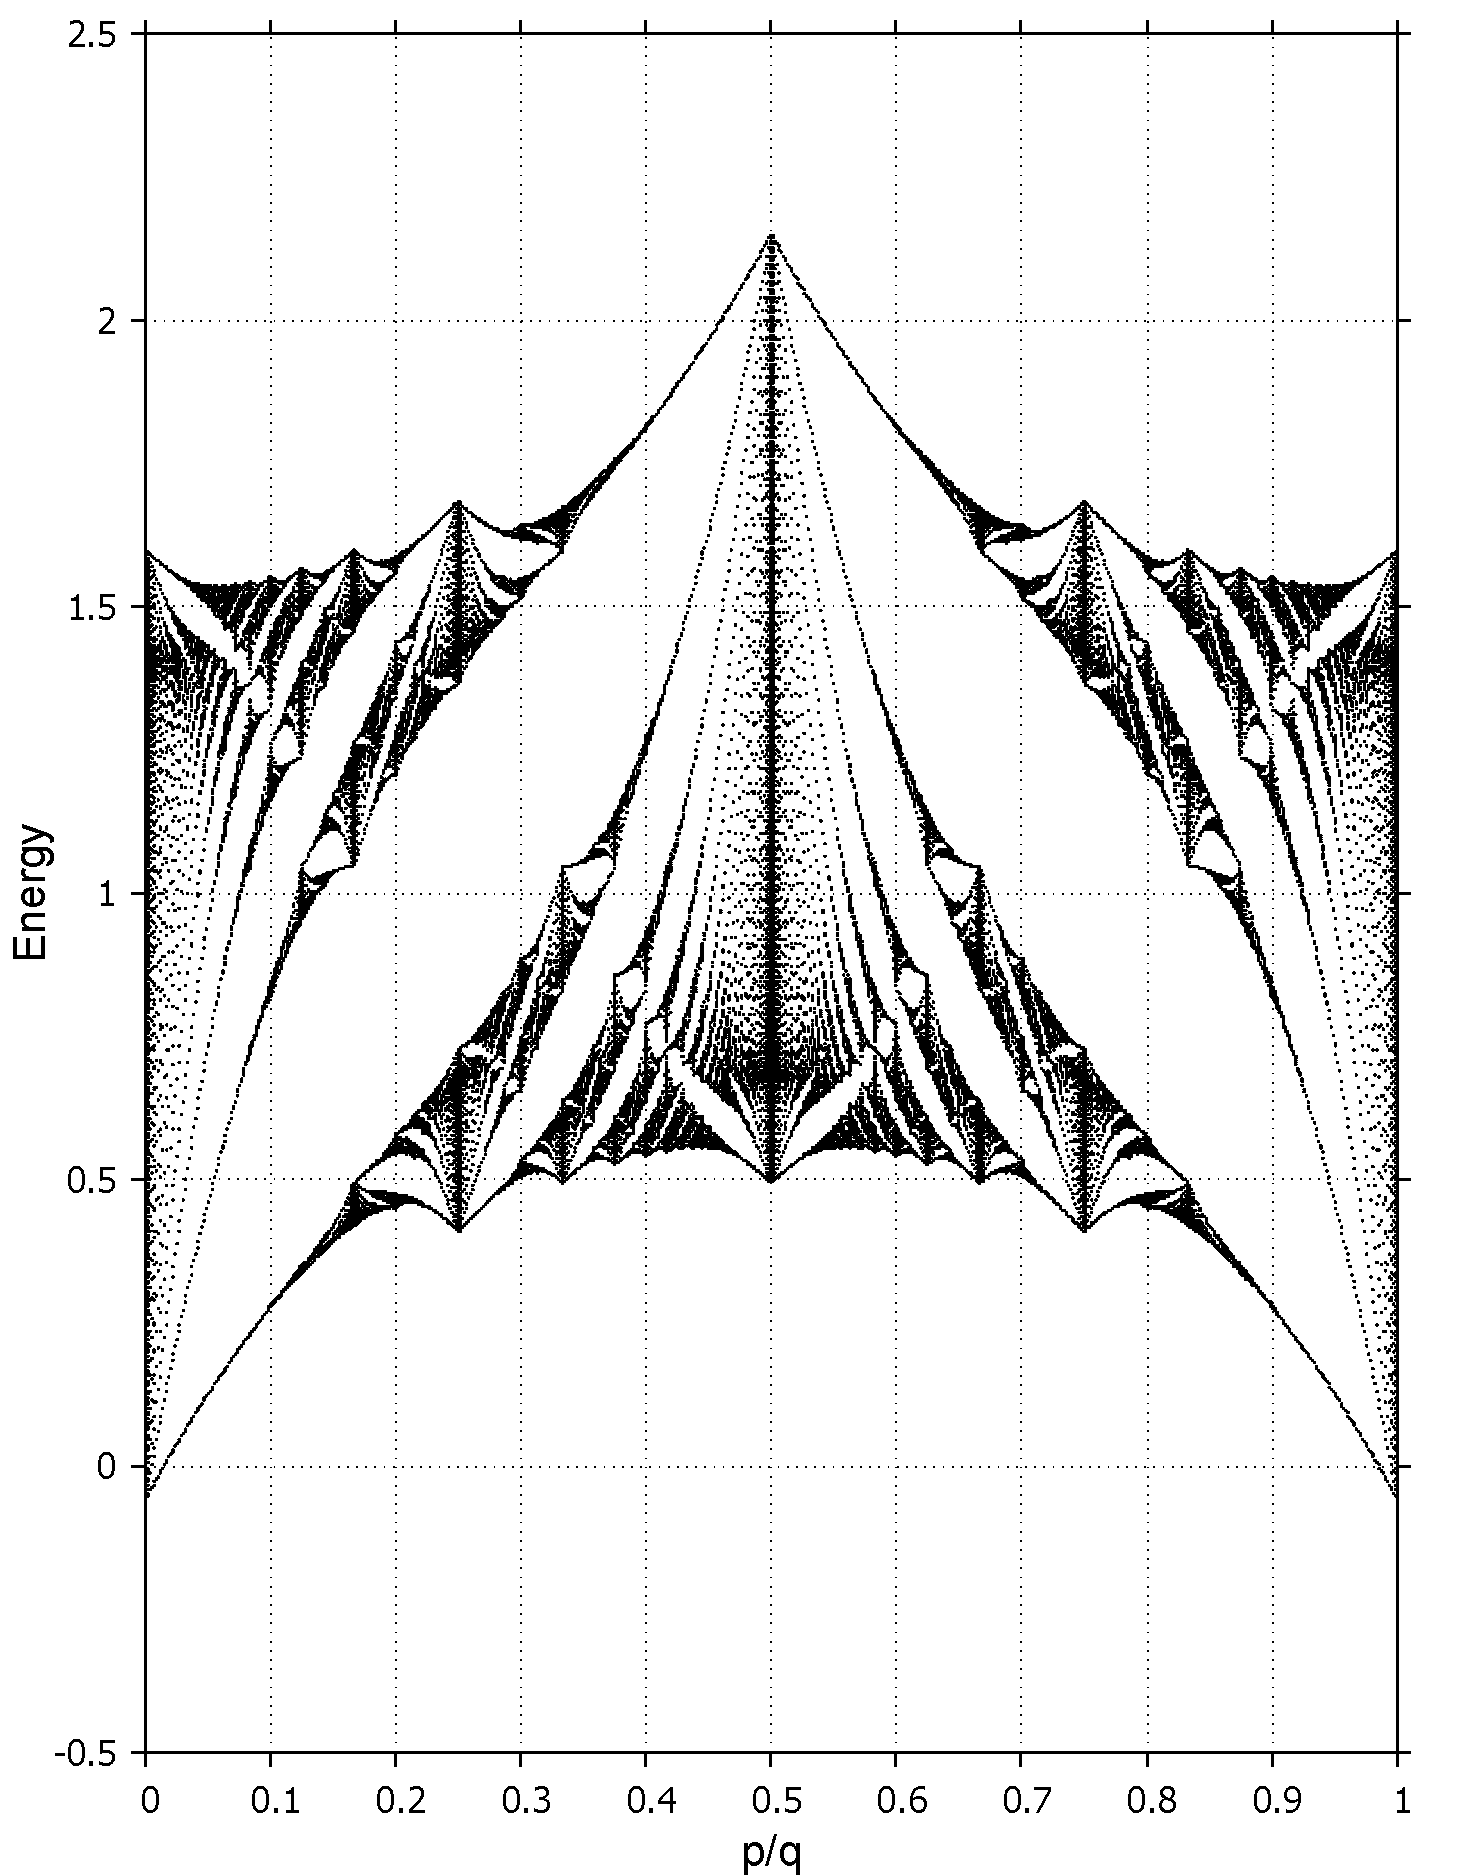
\includegraphics[width=0.6\linewidth]{pic/h0_tam giac_q_797.png}
				\label{fig:3 band}
			\end{subfigure}
			\begin{subfigure}[b]{0.3\textwidth}
				\centering
				\includegraphics[width=0.6\linewidth]{pic/h0_tam giac_TNN_LDA_q_797.png}
				\label{}
			\end{subfigure}
			\begin{subfigure}[b]{0.3\textwidth}
				\centering
				\includegraphics[width=0.6\linewidth]{pic/h0_tam giac_TNN_GGA_q_797.png}
				\label{}
			\end{subfigure}
			\begin{subfigure}[b]{0.3\textwidth}
				\centering
				\includegraphics[width=0.6\linewidth]{pic/3band_gnuplot_TNN_q_797.png}
				\label{fig:1 band}
			\end{subfigure}
			\begin{subfigure}[b]{0.3\textwidth}
				\centering
				\includegraphics[width=0.6\linewidth]{pic/3band_gnuplot_TNN_LDA_q_797.png}
				\label{}
			\end{subfigure}
			\begin{subfigure}[b]{0.3\textwidth}
				\centering
				\includegraphics[width=0.6\linewidth]{pic/3band_gnuplot_TNN_GGA_q_797.png}
				\label{}
			\end{subfigure}
			\caption{
				Hofstadter butterfly for single-band $\ket{dz} \equiv \ket{\phi_{1}^{1}(x,y)}$(left) and three-band(right). 
			}
		\end{figure}
	\end{frame}
 	\begin{frame}{Hofstadter butterfly}
		\begin{multicols}{2}
			\begin{minipage}{\columnwidth}
				\begin{block}{Properties}
					\begin{itemize}
						\item The spectrum depends only on the flux ratio $p/q$.
						\item The spectrum also invariant under reversal of the magnetic field $\tfrac{p}{q} \to -\tfrac{p}{q}$.
						\item The main energy bands are basically Landau levels
						\item At weak magnetic field, Landau levels can clearly seen from the Hofstadter spectrum.
					\end{itemize}
				\end{block}
			\end{minipage}
			\begin{minipage}{\columnwidth}
				\begin{figure}
					\centering
					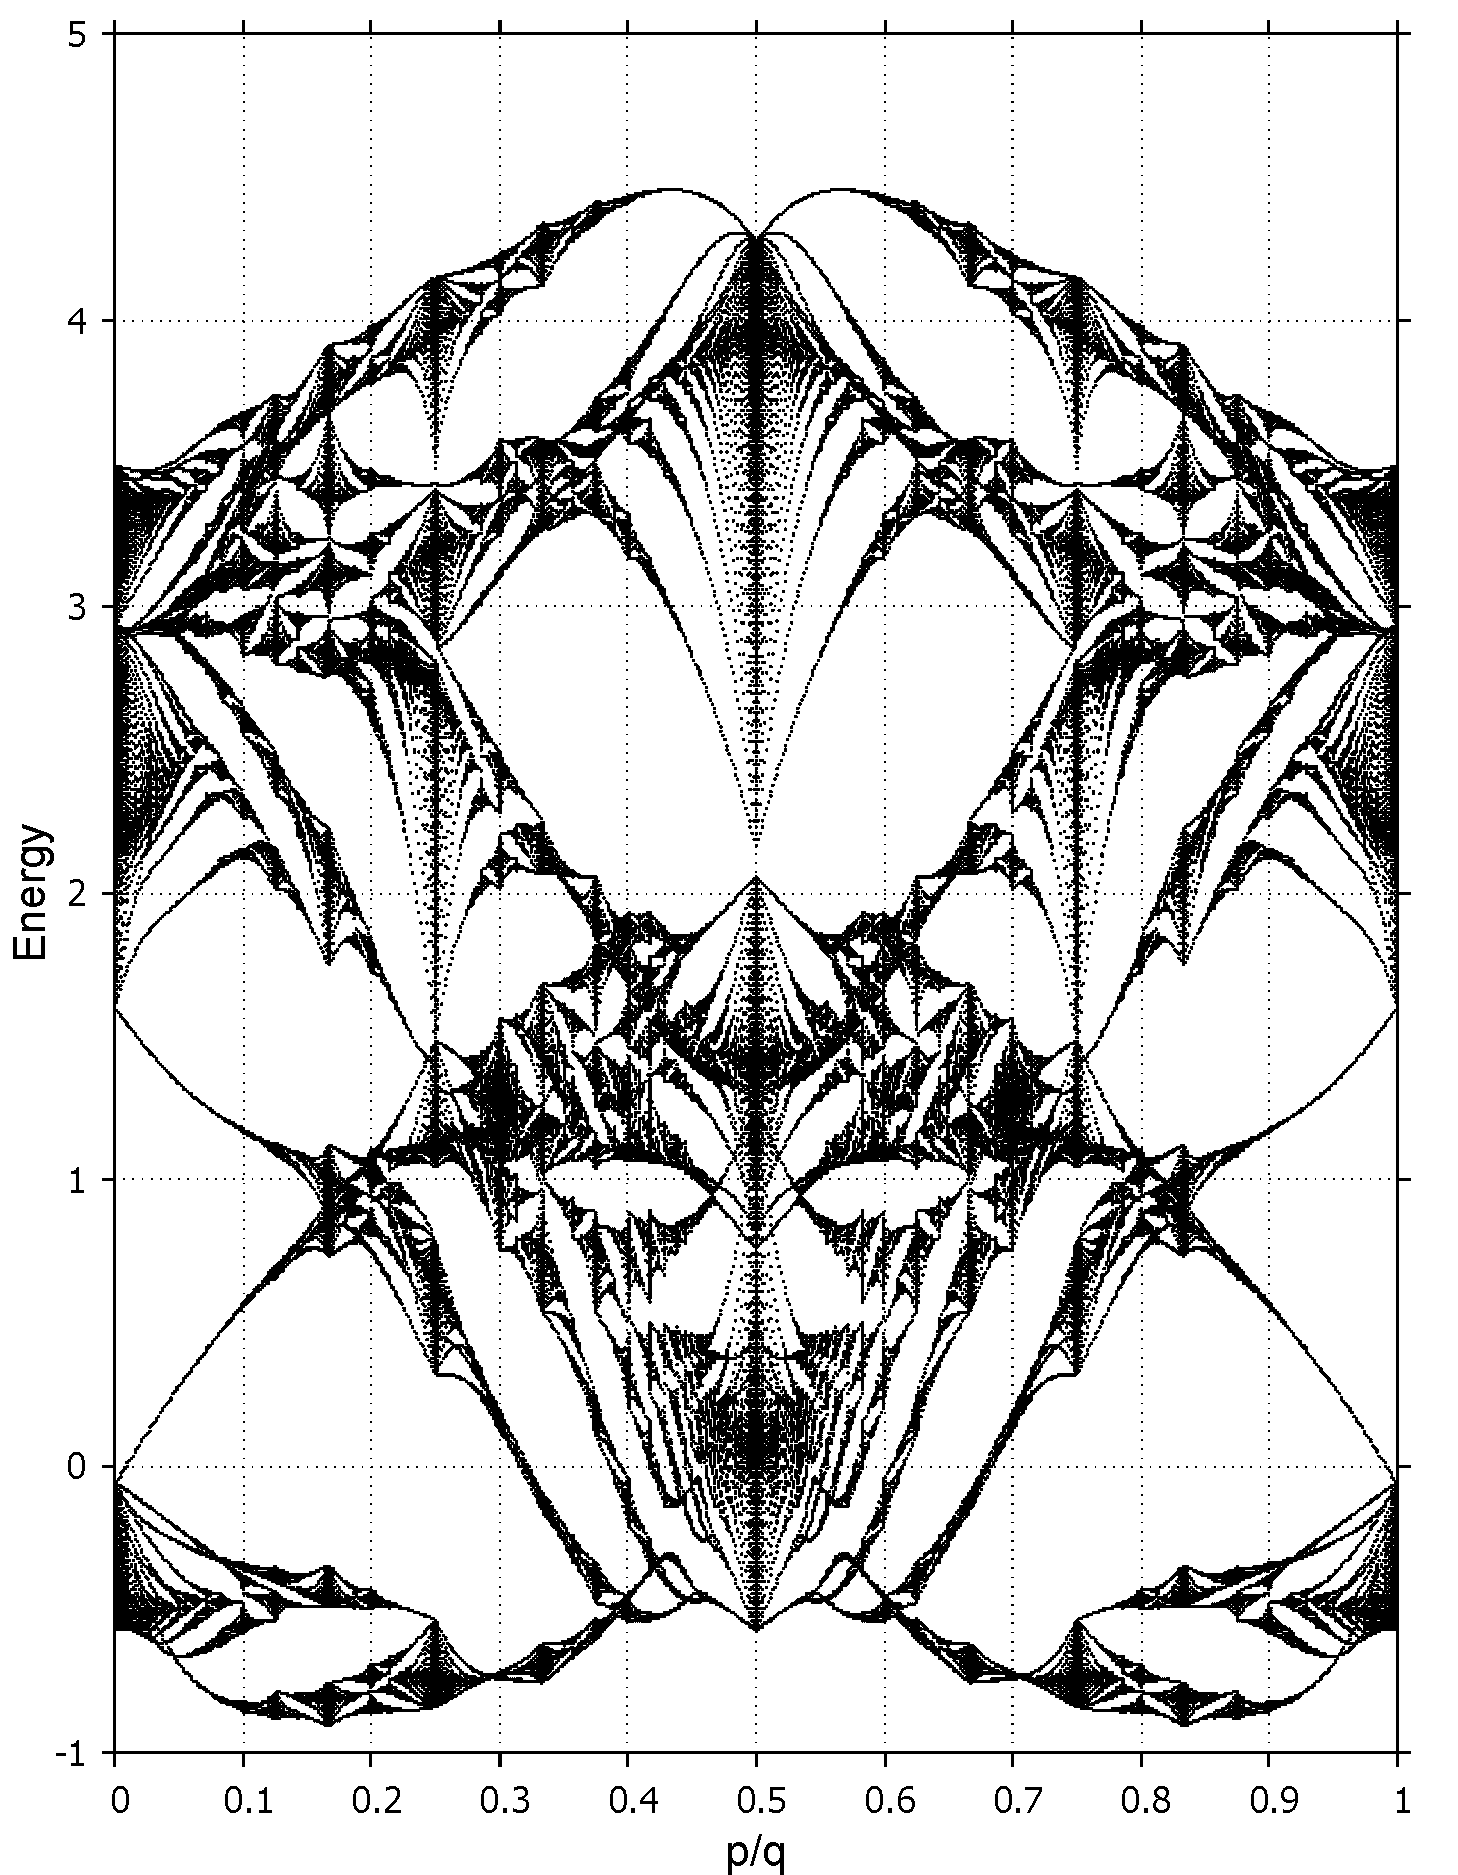
\includegraphics[width=0.65\linewidth]{../pic/3band_gnuplot_q_797.png}
				\end{figure}
			\end{minipage}
		\end{multicols}
	\end{frame}
 	\begin{frame}{Hofstadter butterfly}
		\begin{multicols}{2}
			\begin{minipage}{\columnwidth}
				\begin{block}{Properties}
					\begin{itemize}
						\item The spectrum depends only on the flux ratio $p/q$.
						\item The spectrum also invariant under reversal of the magnetic field $\tfrac{p}{q} \to -\tfrac{p}{q}$.
						\item The main energy bands are basically Landau levels
						\item At weak magnetic field, Landau levels can clearly seen from the Hofstadter spectrum.
					\end{itemize}
				\end{block}
			\end{minipage}
			\begin{minipage}{\columnwidth}
				\begin{figure}
					\centering
					\includegraphics[width=0.65\linewidth]{../TNN/pic/3band_gnuplot_q_797_TNN_LDA.png}
				\end{figure}
			\end{minipage}
		\end{multicols}
	\end{frame}
%	\begin{frame}{Showcase Hofstadter butterflies}
%		\begin{figure}
%			\begin{subfigure}[b]{0.3\linewidth}
%				\centering
%				\includegraphics[width=0.6\linewidth]{../pic/plotHofstadterButterfly_q=797_MoS2.png}
%			\end{subfigure}
%			\begin{subfigure}[b]{0.3\linewidth}
%				\centering
%				\includegraphics[width=0.6\linewidth]{../pic/plotHofstadterButterfly_q=797_MoSe2.png}
%			\end{subfigure}
%			\begin{subfigure}[b]{0.3\linewidth}
%				\centering
%				\includegraphics[width=0.6\linewidth]{../pic/plotHofstadterButterfly_q=797_MoTe2.png}
%			\end{subfigure}
%			\begin{subfigure}[b]{0.3\linewidth}
%				\centering
%				\includegraphics[width=0.6\linewidth]{../pic/plotHofstadterButterfly_q=797_WS2.png}
%			\end{subfigure}
%			\begin{subfigure}[b]{0.3\linewidth}
%				\centering
%				\includegraphics[width=0.6\linewidth]{../pic/plotHofstadterButterfly_q=797_WSe2.png}
%			\end{subfigure}
%			\begin{subfigure}[b]{0.3\linewidth}
%				\centering
%				\includegraphics[width=0.6\linewidth]{../pic/plotHofstadterButterfly_q=797_WTe2.png}
%			\end{subfigure}
%		\end{figure}
%	\end{frame}
	\begin{frame}{Hofstadter butterfly with SOC}
		Three-band TB Hamiltonian under magnetic field with SOC has the form
		\begin{equation}
			\begin{aligned}
				H_{\text{SOC}}(\mathbf{k})
				& =
				\begin{pmatrix}
					H_{3q \times 3q}(\mathbf{k}) + \frac{\lambda}{2} \mathbf{I}_{q} \otimes L_{z} & 0                                                      \\
					0                                                      & H_{3q \times 3q}(\mathbf{k}) - \frac{\lambda}{2} \mathbf{I}_{q} \otimes L_{z}
				\end{pmatrix},
			\end{aligned}
			\begin{aligned}
				L_{z}
				=
				\begin{pNiceMatrix}
					0 & 0   & 0  \\
					0 & 0   & 2i \\
					0 & -2i & 0
				\end{pNiceMatrix}
			\end{aligned}
		\end{equation}
	\end{frame}
	\begin{frame}{Bandstructure of TMD with SOC}
		\begin{figure}
			\begin{subfigure}[b]{0.495\textwidth}
				\centering
				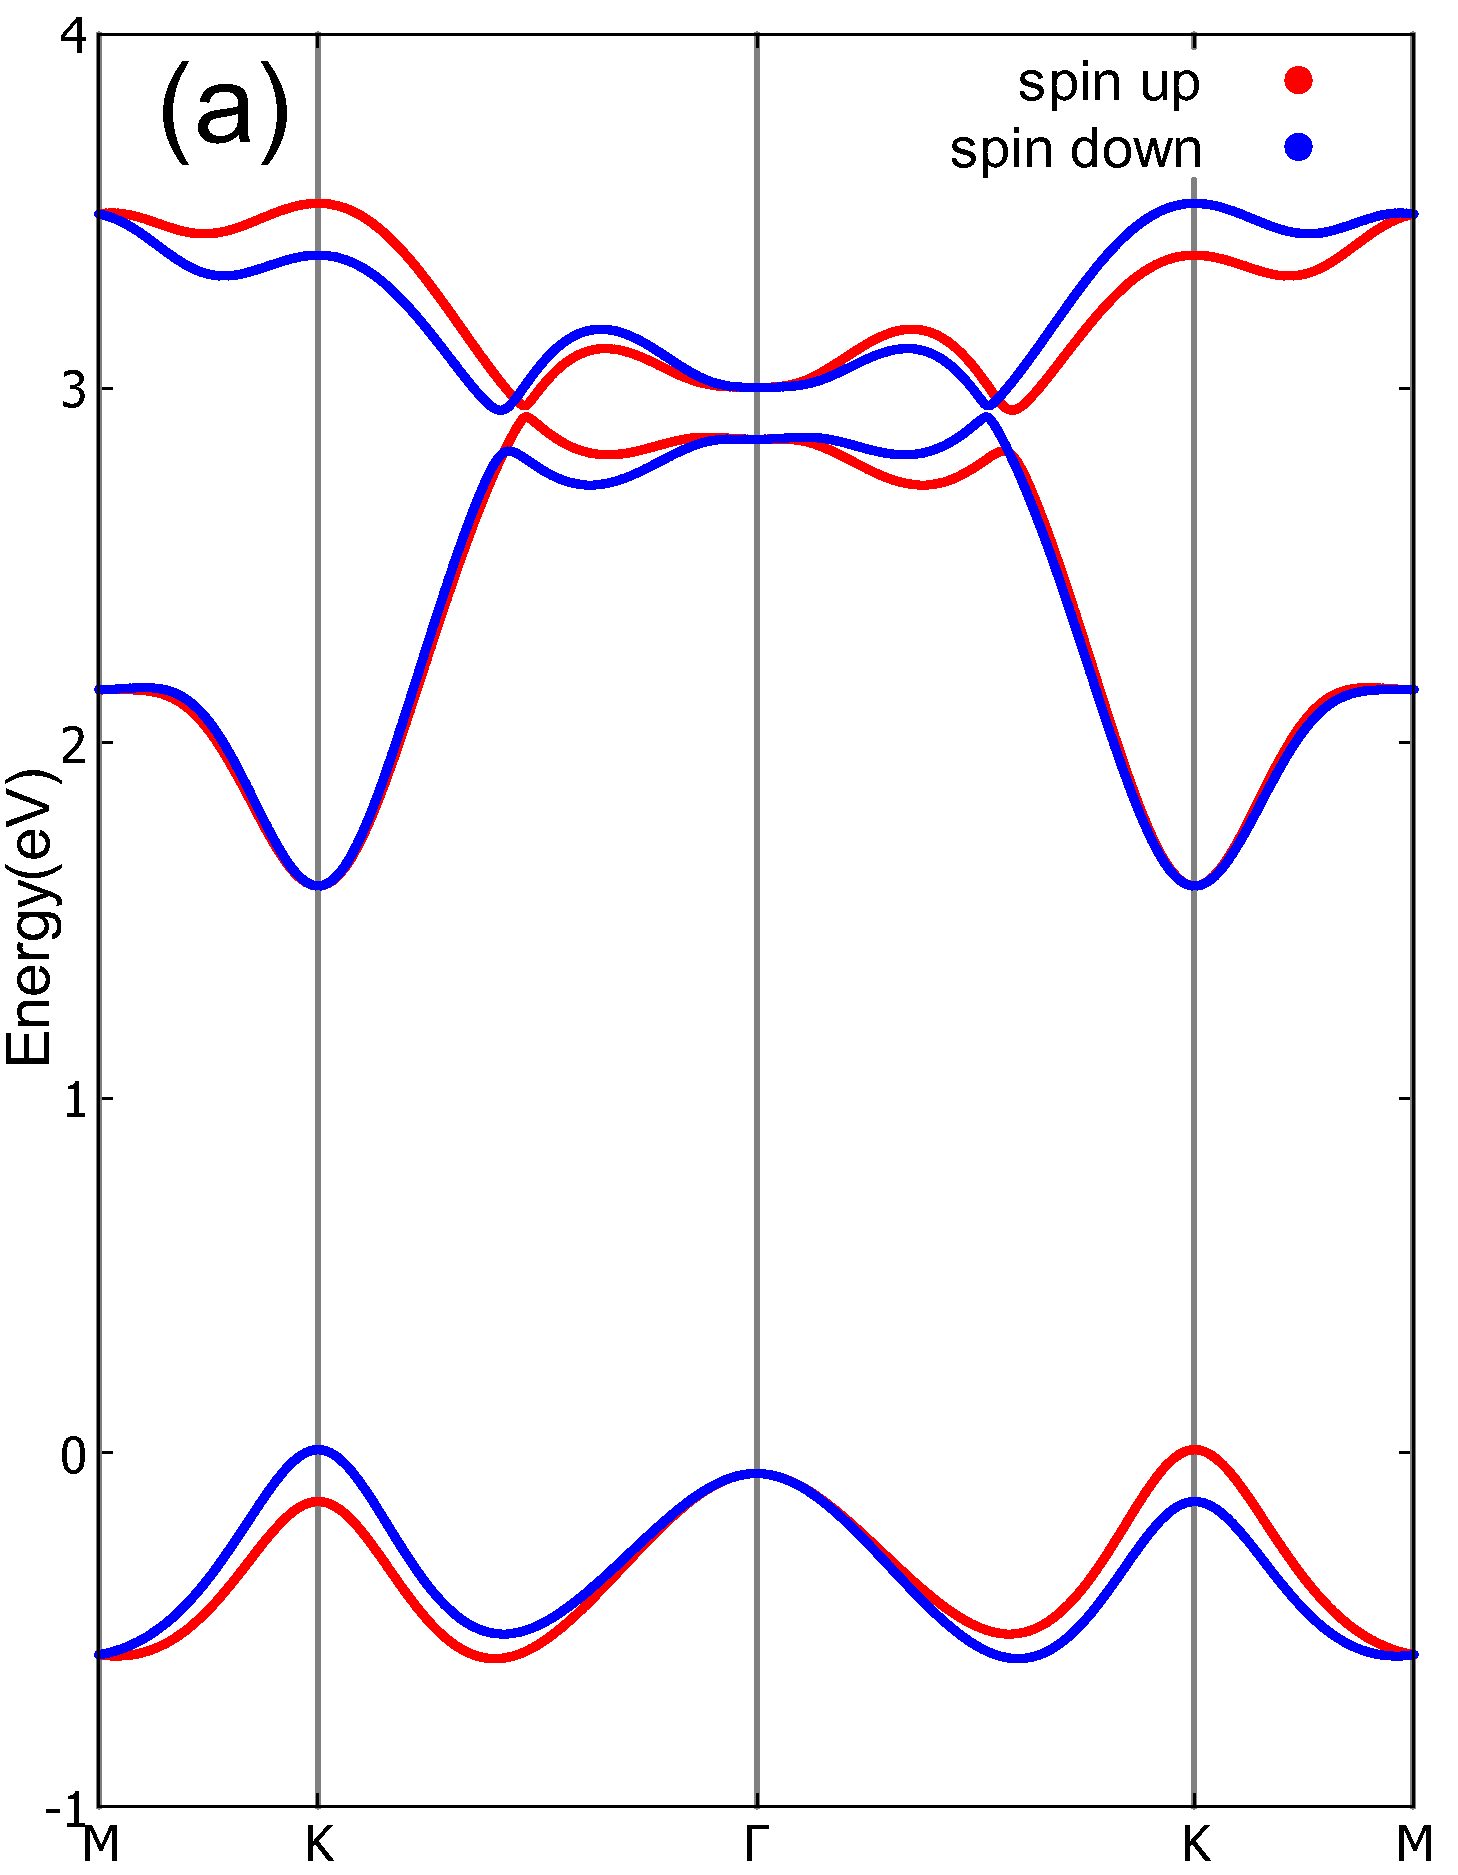
\includegraphics[width=0.6\linewidth]{pic/bandstructureSOC.pdf}
				%\caption{\label{band structure SOC}}
			\end{subfigure}
			\begin{subfigure}[b]{0.495\textwidth}
				\centering
				\includegraphics[width=0.6\linewidth]{pic/bandstructureSOCTNN.pdf}
				%\caption{\label{HB SOC}}
			\end{subfigure}
			\caption{Band structure of monolayer MoS$_{2}$ along $\Gamma$-K direction with SOC.}
		\end{figure}
	\end{frame}
	\begin{frame}{Hofstadter butterfly with SOC}
		\begin{figure}
			\begin{subfigure}[b]{0.495\textwidth}
				\centering
				\includegraphics[width=0.6\linewidth]{pic/plotHofstadterButterfly_q=797_MoS2_SOC_f.png}
				%\caption{\label{band structure SOC}}
			\end{subfigure}
			\begin{subfigure}[b]{0.495\textwidth}
				\centering
				\includegraphics[width=0.6\linewidth]{pic/plotHofstadterButterfly_q=797_MoS2_SOC_LDA.png}
				%\caption{\label{HB SOC}}
			\end{subfigure}
			\caption{Hofstadter butterfly with SOC.}
		\end{figure}
	\end{frame}
	
	\subsection{Landau levels}
	\begin{frame}{Landau levels}
		The Hamiltonian for free-electron
		\begin{gather}
			H = \frac{\mathbf{p} + e \mathbf{A}(\mathbf{r})^{2}}{2m} ,
		\end{gather}
		and the energy eigenfunctions are known as Landau levels
		\begin{gather}
			E_{n} = \left(n + 1/2\right) \hbar \omega_{c},
		\end{gather}
		where $\omega_{c}$ is cyclotron frequency and $n$ is Landau level index.
	\end{frame}
	\begin{frame}{Envelope Function Approximation}
		The dispersion relation of an electron within TBM
		\begin{equation}
			\begin{aligned}
				H_{11} 
				& \approx 6 t_{0} - \frac{3}{2} t_{0} a^{2} (k_{x}^{2} + k_{y}^{2}) + \epsilon_{1}.
			\end{aligned}
		\end{equation}
		Using Envelop Function Approxmation (EFA) substitution $\hbar\mathbf{k} \to \mathbf{\Pi} + e \mathbf{A}$ with Landau gauge $\mathbf{A} = (0,Bx,0)$
		\begin{gather}
			H_{11}(\mathbf{\Pi})
			\approx 6 t_{0} - \frac{3}{2} t_{0} \frac{a^{2}}{\hbar^{2}} \left[ \Pi_{x}^{2} + \left(\Pi_{y} + e B x\right)^{2}\right] + \epsilon_{1}.
		\end{gather}
		Eq. (21) can be rewrite in the form as 
		\begin{gather}
			E(\mathbf{\Pi}) = 6 t_{0} - \left[\frac{1}{2m^{*}} \Pi_{x}^{2} + \frac{1}{2} m^{*} \omega_{c}^{2}(x - x_{0})^{2}\right] + \epsilon_{1},
		\end{gather}
		where $m^{*} = \frac{\hbar^{2}}{3t_{0}a^{2}}$ is the effective mass and $x_{0} = \frac{\hbar k_{y}}{eB}$. Subsequently, the cyclotron frequency is
		\begin{gather}
			\omega_{c} = \frac{eB}{m^{*}} = \frac{8 \pi \sqrt{3} t_{0}}{\hbar}  \frac{p}{q},
		\end{gather}
	\end{frame}
	\begin{frame}{Landau Level}
		and therefore the Landau levels near the bottom of the band structure can be written as
		\begin{equation}
			\begin{aligned}
				E_{n}
				& = 6 t_{0} - \hbar \omega_{c} (n + 1 /2) + \epsilon_{1}                    \\
				& = t_{0} \left(6 - 8\pi\sqrt{3} \frac{p}{q}( n + 1 /2)\right) + \epsilon_{1}.
			\end{aligned}
		\end{equation}
		Plot Eq. (25) while varrying $p$ from $1\to q$ which Landau level index $n$ we get
	\end{frame}
	\begin{frame}{Landau levels}
		\begin{figure}
			\centering
			\begin{subfigure}[b]{0.49\textwidth}
				\centering
				{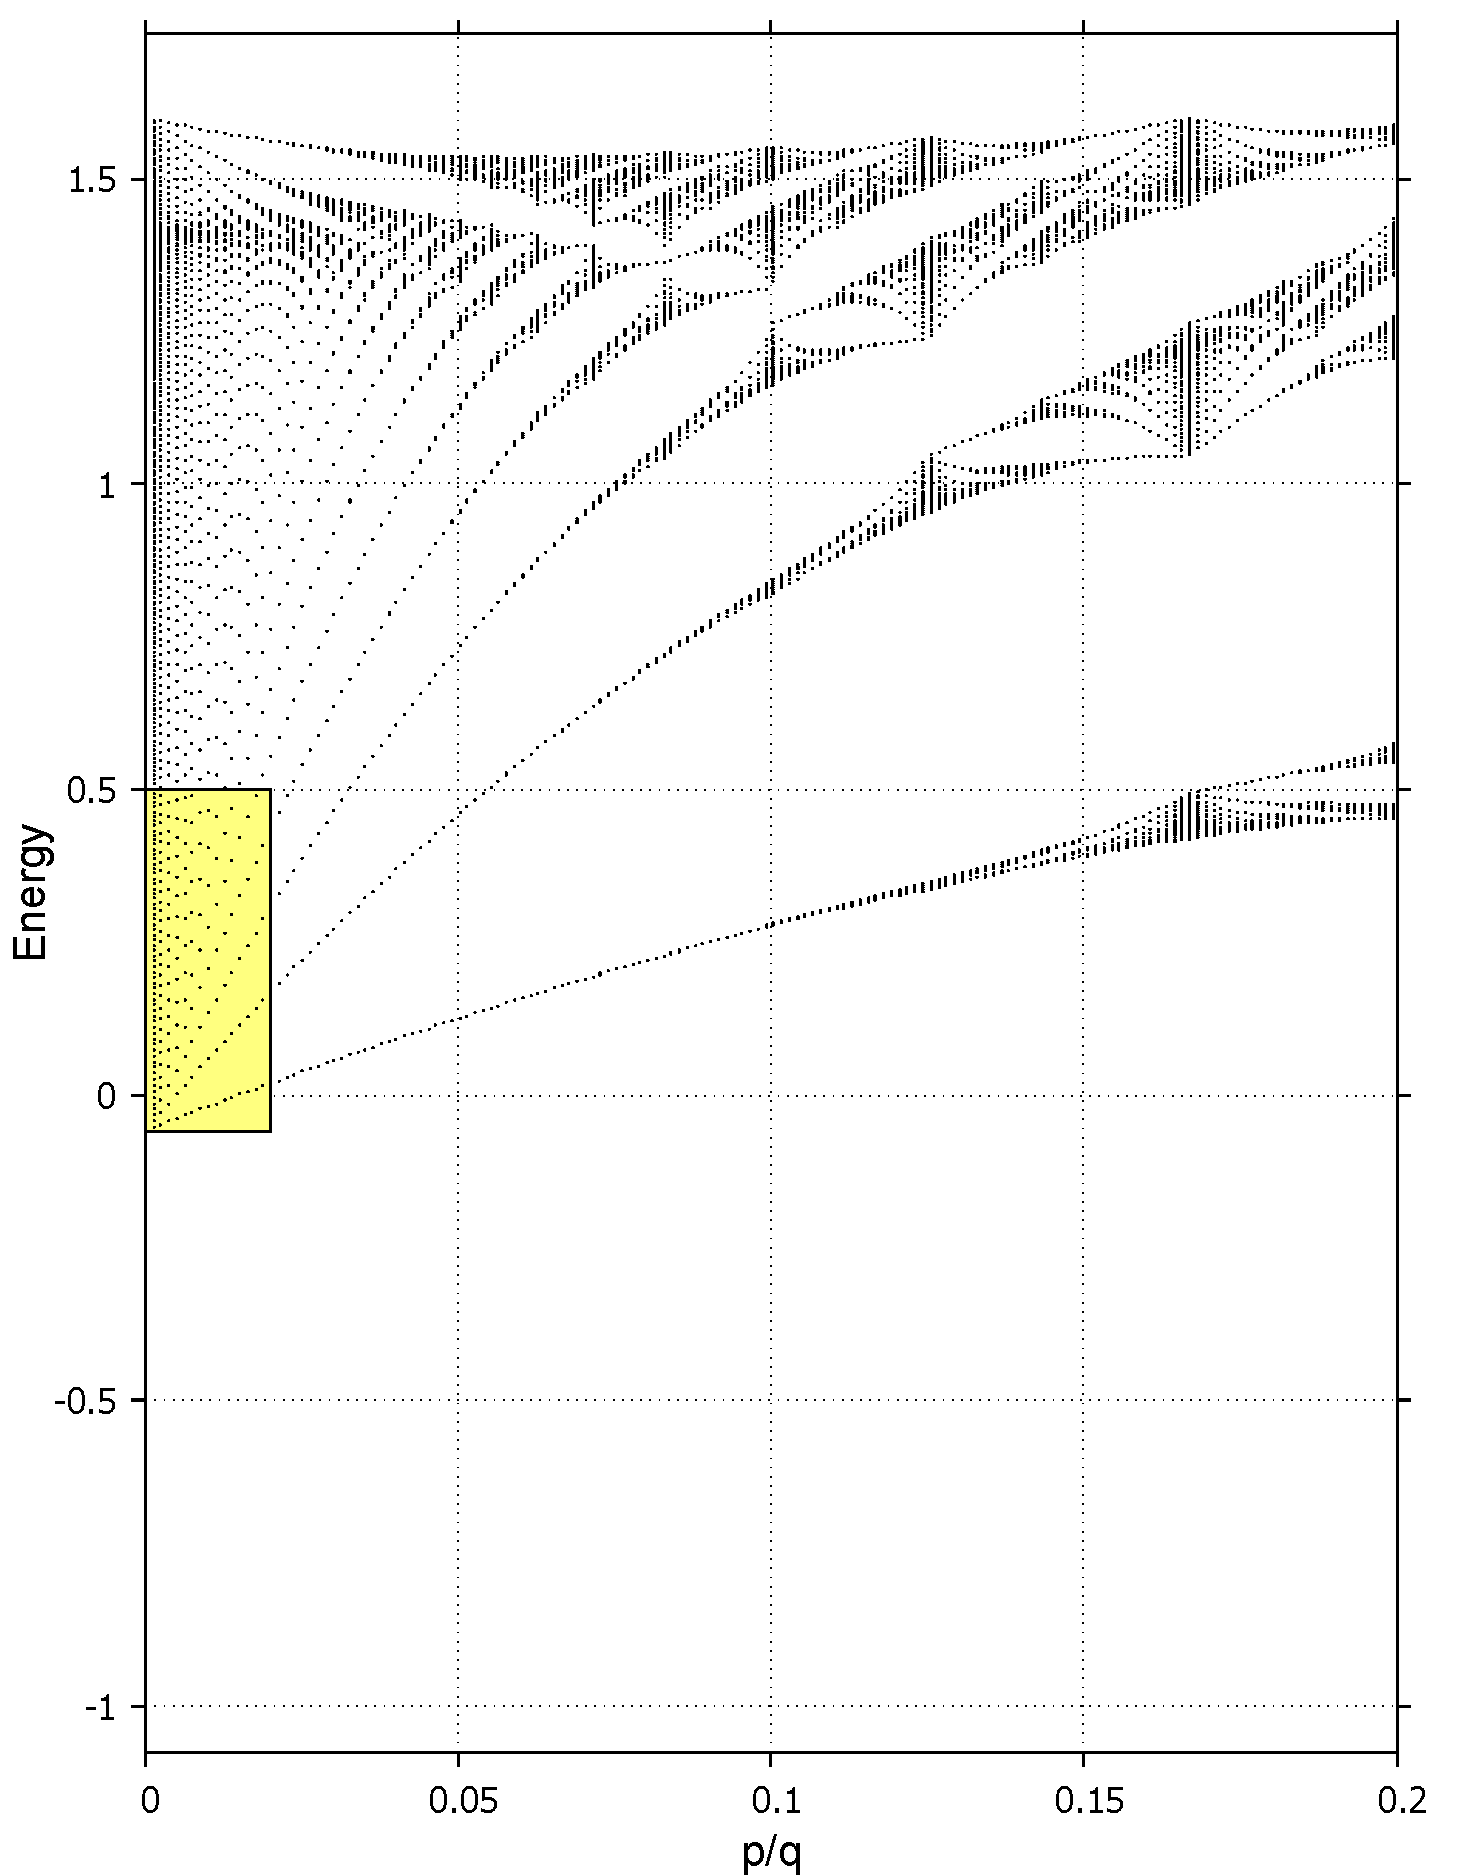
\includegraphics[width=0.6\linewidth]{../pic/small_area_LL.png}}
			\end{subfigure}
			\hspace{-3\baselineskip}
			\begin{subfigure}[b]{0.49\textwidth}
				\centering
				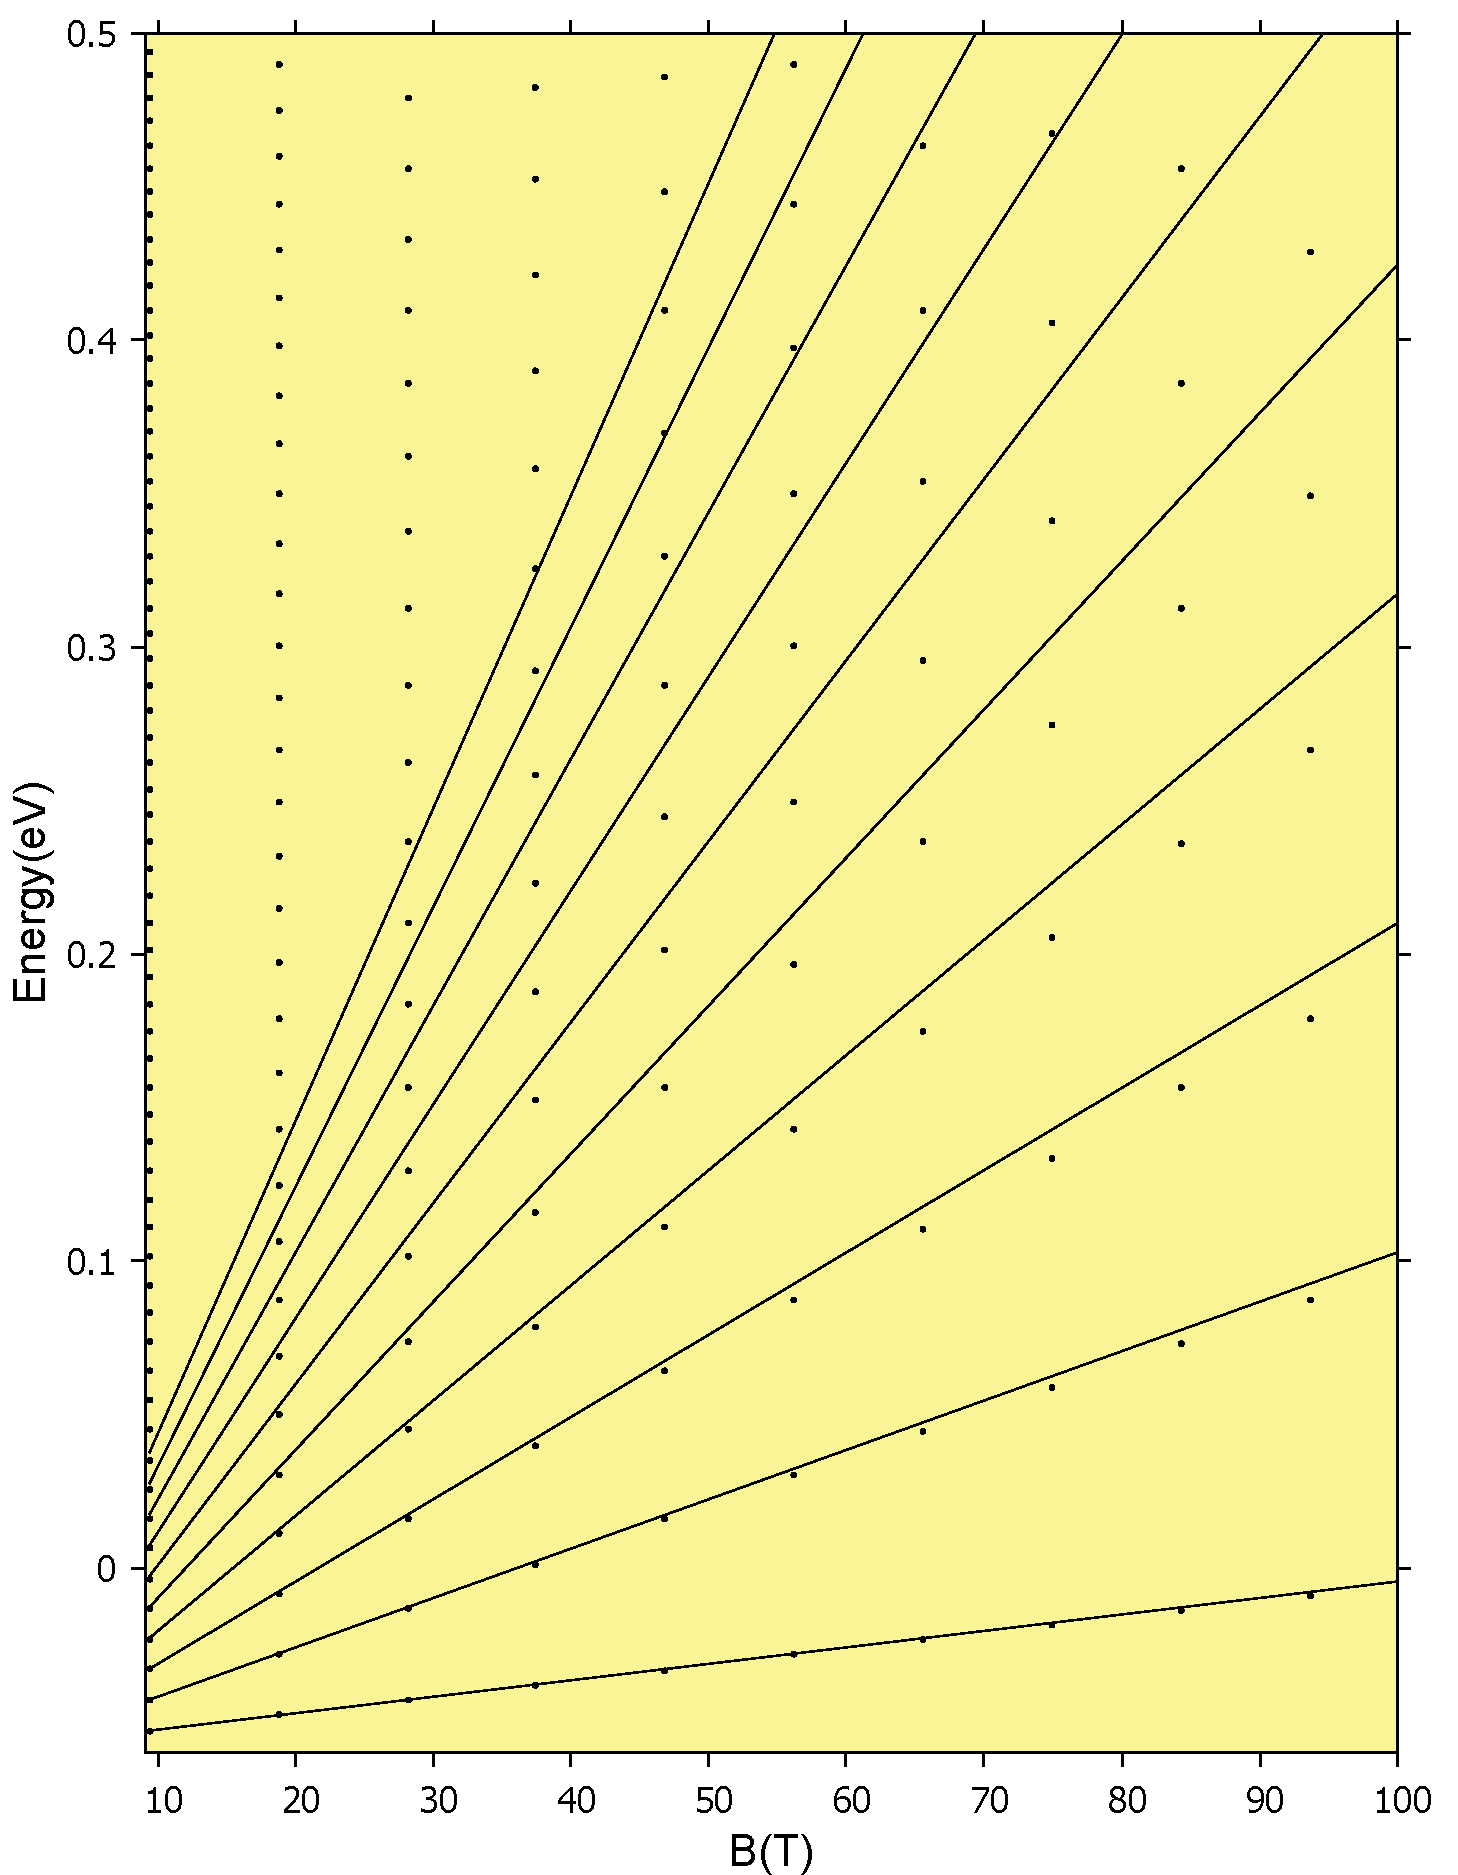
\includegraphics[width=0.6\linewidth]{../pic/landaulevel_h0_q_797.pdf}
			\end{subfigure}
			\caption{
				Landau levels appear in weak magnetic field.
			}
		\end{figure}
	\end{frame}
	\begin{frame}{Landau levels}
		\begin{multicols}{2}
			\begin{minipage}{\columnwidth}
				\begin{figure}
					\centering
					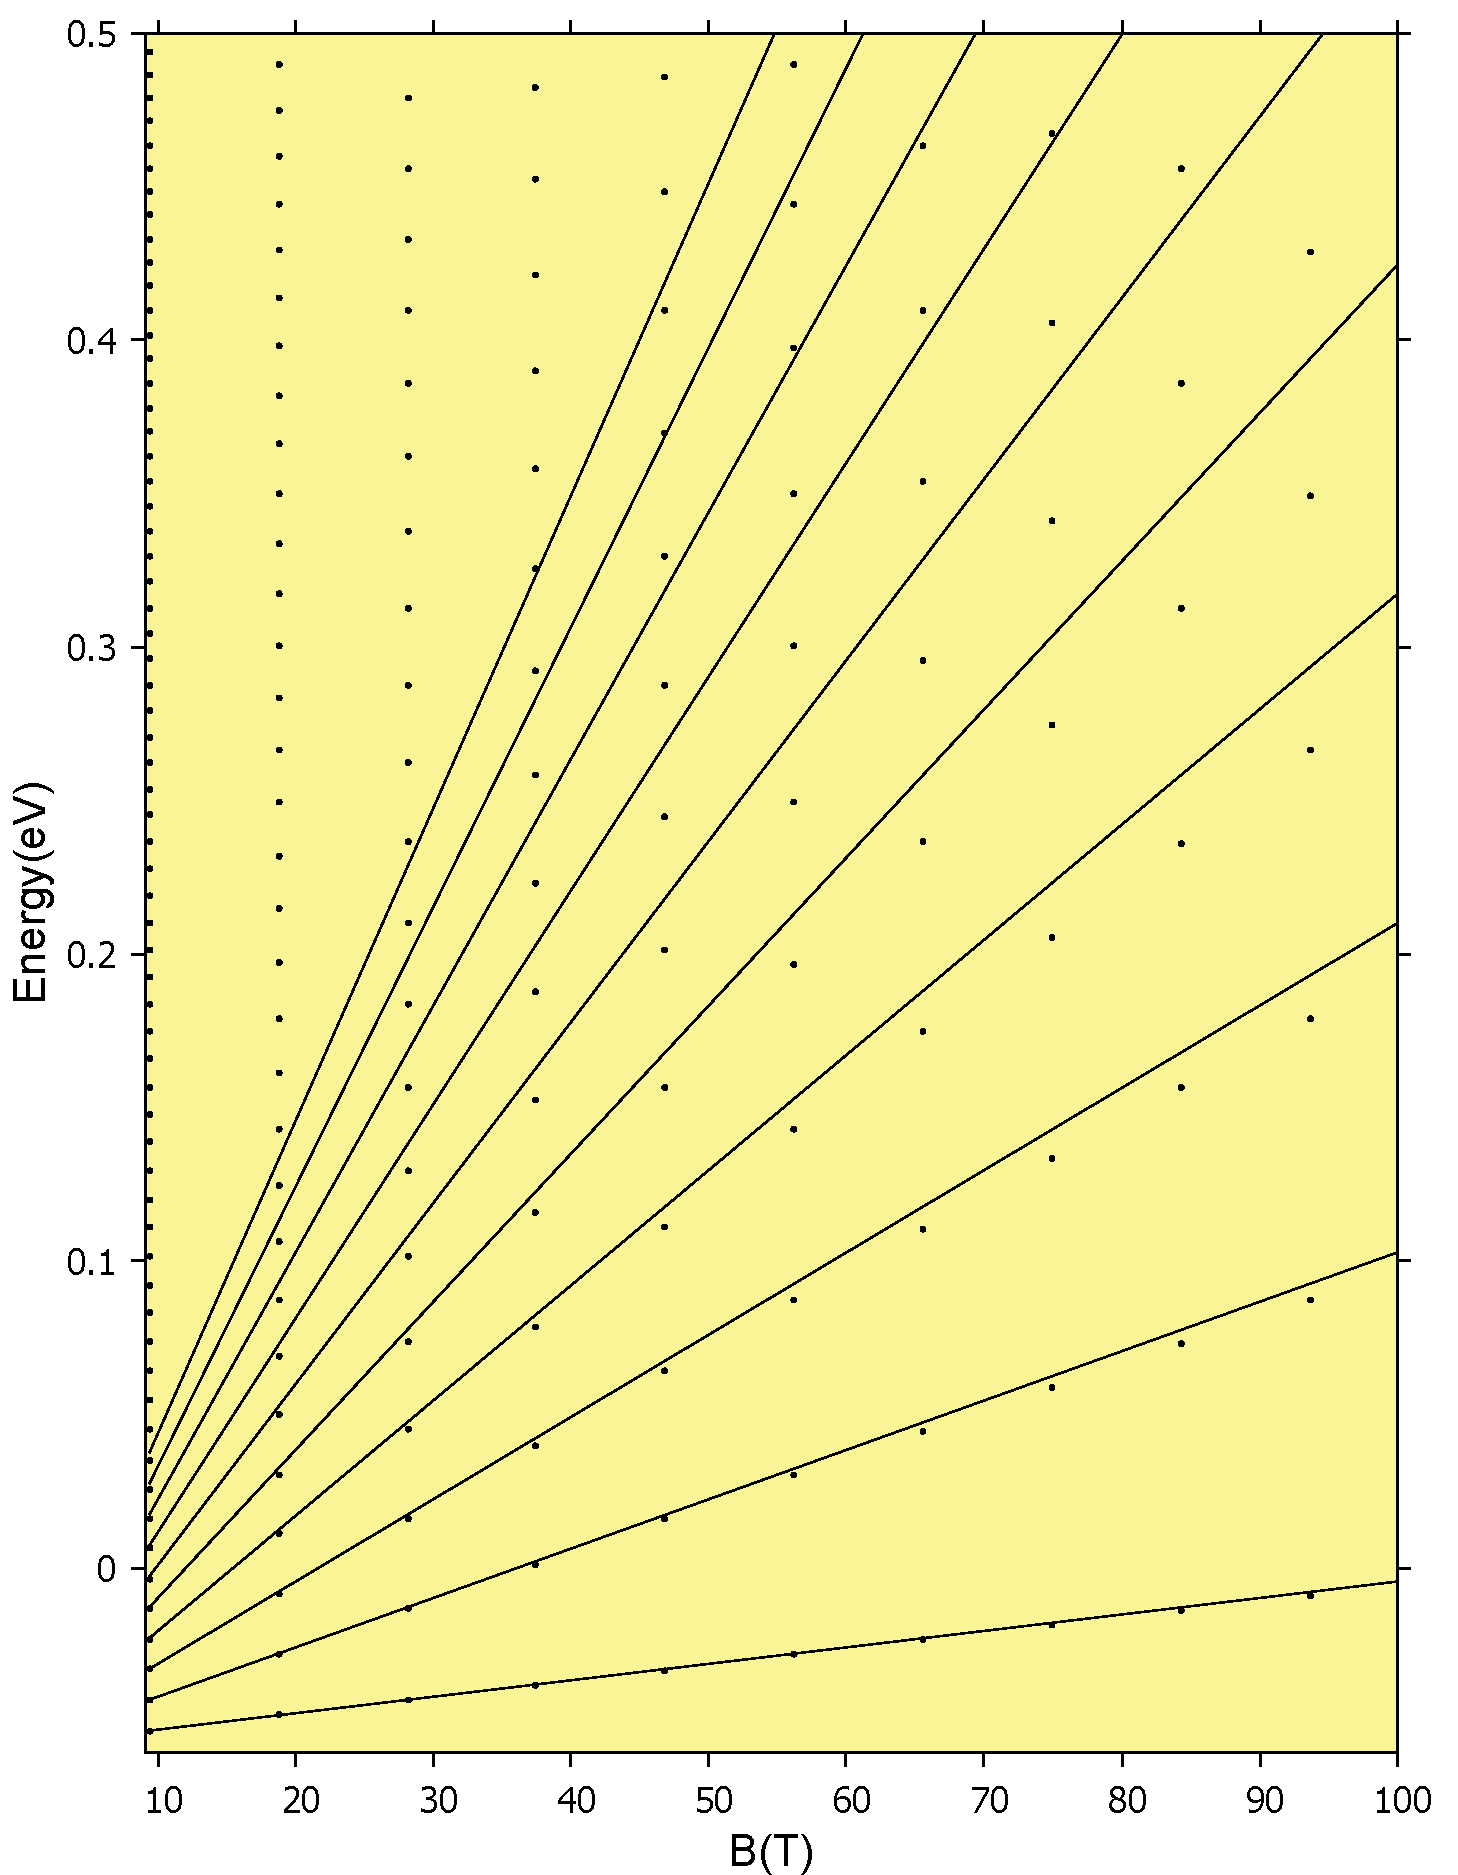
\includegraphics[width=0.7\linewidth]{../pic/landaulevel_h0_q_797.pdf}
				\end{figure}
			\end{minipage}
			\begin{minipage}{\columnwidth}
				\begin{block}{Properties}
					\begin{itemize}
						\item Increase linearly with respect to $B$.
						\item At weak magnetic field, the Landau levels are well-described.
						\item Increasing $B$ $\to$ fewer filled levels.
						\item At extremely strong field $\to$ only one level is filled.
					\end{itemize}
				\end{block}
			\end{minipage}
		\end{multicols}
	\end{frame}
	\subsection{Hall effect}
	\begin{frame}{The Classical Hall effect}
		\begin{multicols}{2}
			\begin{figure}
				\centering
				\includegraphics[width=0.8\linewidth]{../pic/HEsetup.png}
				\caption{Classical Hall effect}
			\end{figure}
			\columnbreak
			The Hall effect can be described through Ohm's law
			\begin{gather}
				\begin{pNiceMatrix}
					J_{x} \\
					J_{y}
				\end{pNiceMatrix}
				=
				\begin{pNiceMatrix}
					\sigma_{xx} & \sigma_{xy} \\
					\sigma_{yx} & \sigma_{yy} \\
				\end{pNiceMatrix}
				\begin{pNiceMatrix}
					E_{x} \\
					E_{y}
				\end{pNiceMatrix}, \\
				\begin{pNiceMatrix}
					E_{x} \\
					E_{y}
				\end{pNiceMatrix}
				=
				\begin{pNiceMatrix}
					\rho_{xx} & \rho_{xy} \\
					\rho_{yx} & \rho_{yy} \\
				\end{pNiceMatrix}
				\begin{pNiceMatrix}
					J_{x} \\
					J_{y}
				\end{pNiceMatrix}.
			\end{gather}
		\end{multicols}
		\begin{figure}
			\begin{subfigure}[b]{0.4\textwidth}
				\centering
				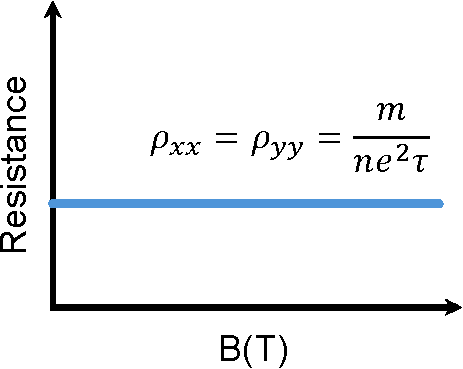
\includegraphics[width=0.6\linewidth]{../pic/classRess.pdf}
			\end{subfigure}
			\hspace{-3\baselineskip}
			\begin{subfigure}[b]{0.4\textwidth}
				\centering
				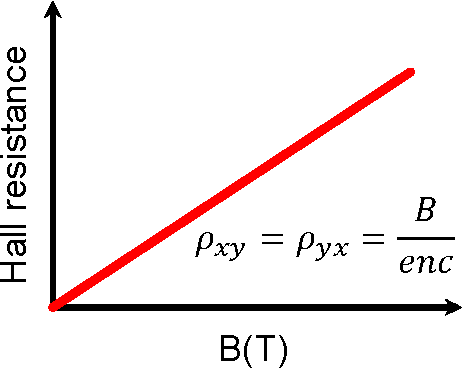
\includegraphics[width=0.6\linewidth]{../pic/HallRess.pdf}
			\end{subfigure}
		\end{figure}
	\end{frame}
	\begin{frame}{The Quantum Hall effect}
		\begin{multicols}{2}
			It was first discovered in early 1980\footnotemark. \\
			The resistance in a MOSFET under a strong magnetic field depicts interesting phenomena.
			\begin{minipage}{\columnwidth}
				\begin{block}{Properties}
					\begin{itemize}
						\item On Hall plateaux
						\begin{gather*}
							\rho_{xx} = \rho_{yy} = 0, \quad \rho_{xy} = \rho_{yx} = \fontfamily{serif}\text{const}.\\
							\sigma_{xx} = \sigma_{yy} = 0, \quad \sigma_{xy} = \sigma_{yx} = 1/ \fontfamily{serif}\text{const}.
						\end{gather*}
						\item Between Hall plateaux
						\begin{gather*}
							\rho_{xx},\rho_{yy} \neq 0 \Rightarrow \sigma_{xx},\sigma_{yy} \neq 0, \\
							\rho_{xy} = \tfrac{R_{K}}{\nu}, \quad \nu = 1,2,3,...
						\end{gather*}
					\end{itemize}
				\end{block}
			\end{minipage}
			\columnbreak
			\begin{figure}
				\centering
				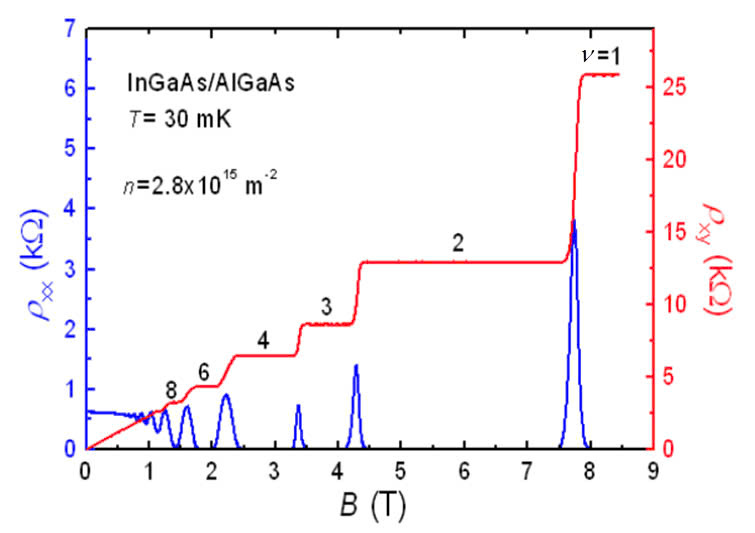
\includegraphics[width=0.95\linewidth]{../pic/quantumhall.jpg}
				\caption{The Quantum Hall effect by \citeauthor{klitzing90} (\citeyear{klitzing90}).}
			\end{figure}
			%\footnotetext{\citeauthor{klitzing90}}
		\end{multicols}
	\end{frame}
	\begin{frame}{The Quantum Hall effect}
		The contribution to the Hall conductance is given by
		\begin{gather}
			\sigma_{xy} = \frac{e^{2}}{h} \sum_{n}^{\fontfamily{seriff}\text{occ.}} \frac{1}{2\pi} \oiint_{\fontfamily{serif}\text{{BZ}}} d k_{x} d k_{y} \Omega_{n}^{z} (\mathbf{k}),
		\end{gather}
		since the integral over the Brillouin zone is an integer, we arrived at the TKNN formula \footcite{thouless1982}
		\begin{gather}
			\sigma_{xy} = \frac{e^{2}}{h} \nu, \quad \nu = 1,2,...
		\end{gather}
		and combine with Streda formula \footcite{streda1982}
		\begin{gather}
			\sigma_{xy}(B,E_{F}) = e \frac{\partial N (E,B)}{\partial B} \at{E=E_{F}}{},
		\end{gather}
		we have the Diophantine equation
		\begin{gather}
			r = q \times s_{r} + p \times \nu_{r}.
		\end{gather}
	\end{frame}
	\begin{frame}{The Diophantine equation}
		\begin{table}
			\begin{equation*}
				\renewcommand{\arraystretch}{1.1}
				\begin{NiceArray}{ c  c  c  c  c  c  c  c  c  c  c  c  c c}
					\hline
					\hline
					{r} & 0 & 1  & 2  & 3  & 4                & 5  & 6  & 7  & 8 & 9                 & 10 & 11 & 12\rule{0pt}{0.1em} \\
					\hline \hline
					{\nu} & 0 & -3 & -6 & 4  & \color{purple}{1} & -2 & -5 & 5  & 2 & \color{purple}{-1} & -4 & -6 & 3                   \\
					\hline
					s   & 0 & 1  & 2  & -1 & 0                & 1  & 2  & -1 & 0 & 1                 & 2  & -1 & 0                   \\
					\hline
					\hline
				\end{NiceArray}
			\end{equation*}
			\caption[Values of Chern numbers.]{Allowed values of $r$.}
		\end{table}
		\begin{gather*}
			{\color{orange}r} = {\color{green}q} \times {\color{blue}s}{\color{orange}_{r}} + {\color{green}p} \times {\color{red}\nu}\color{orange}{_{r}}.
		\end{gather*}
		\begin{multicols}{2}
			\begin{itemize}
				\item $\color{green}p,q$ are the flux number $\Phi$ and flux quanta $\Phi_{0}$.
				\item The Chern number $\color{red}\nu$ determines the topological and the contribution to the Hall conductance.
				\columnbreak
				\item  Identifying ${\color{blue}s}$ as an index of energy gap in the butterfly. 
				\item {$\color{orange}{r}$} is goes from $0$ to $q-1$ subbands
			\end{itemize}
		\end{multicols}
	\end{frame}
	\begin{frame}{Color the butterfly}
		\begin{figure}
			\captionsetup{labelformat=empty}
			\centering
			\begin{subfigure}[b]{0.495\textwidth}
				\centering
				{\includegraphics[width=0.7\linewidth]{../TNN/pic/1band_Chern_q_199_f.pdf}}
			\end{subfigure}
			\begin{subfigure}[b]{0.495\textwidth}
				\centering
				\includegraphics[width=0.7\linewidth]{../pic/3band_Chern_q_199_f.png}
			\end{subfigure}
			\caption{${\color{orange}r} = {\color{green}q} \times {\color{blue}s}{\color{orange}_{r}} + {\color{green}p} \times {\color{red}\nu}\color{orange}{_{r}}$}
		\end{figure}
	\end{frame}
	\begin{frame}{Color the butterfly}
		\begin{figure}
			\captionsetup{labelformat=empty}
			\centering
			\begin{subfigure}[b]{0.495\textwidth}
				\centering
				{\includegraphics[width=0.7\linewidth]{../TNN/pic/1band_Chern_q_797_colorplane2.png}}
			\end{subfigure}
			\begin{subfigure}[b]{0.495\textwidth}
				\centering
				\includegraphics[width=0.7\linewidth]{../TNN/pic/3band_Chern_q_797_colorplane_f.png}
			\end{subfigure}
			\caption{${\color{orange}r} = {\color{green}q} \times {\color{blue}s}{\color{orange}_{r}} + {\color{green}p} \times {\color{red}\nu}\color{orange}{_{r}}$}
		\end{figure}
	\end{frame}
	\section{Summary and Outlook}
	\begin{frame}
		\begin{block}{Summary:}
			\begin{itemize}
				\item We confirm the Hofstadter butterfly in this model corrected compared to previous study.\\
				\item From three-band TB + magnetic field $\to$ QHE.
			\end{itemize}
		\end{block}
		\begin{exampleblock}{Further research:}
			\begin{itemize}
				\item Fractional Quantum Hall effect
				\item High Harmonic Generation
				\item High-order Side-band Generation
				\item Photovoltaic effect
			\end{itemize}
		\end{exampleblock}
		\begin{multicols}{2}
			\begin{center}
				\null\vfill
				Thank you for your listening.
				\null\vfill
			\end{center}\columnbreak
		\end{multicols}
		\note[item]{So far, we have used the three-band tight-binding model and semiconductor Bloch equations to calculate the linear absorption spectrum. We confirm that this model matches the results with the experiment data and also predicts smaller exciton peaks.}
		\note[item]{For further results, we can include the many-body interaction in calculating other phenomena for a realistic picture of TMD's properties.}
	\end{frame}
	\begin{frame}{References}
		\printbibliography
	\end{frame}
\end{document}